% Options for packages loaded elsewhere
\PassOptionsToPackage{unicode}{hyperref}
\PassOptionsToPackage{hyphens}{url}
\PassOptionsToPackage{dvipsnames,svgnames,x11names}{xcolor}
%
\documentclass[
  letterpaper,
  oneside,
  openany]{MastersDoctoralThesis}

\usepackage{amsmath,amssymb}
\usepackage{iftex}
\ifPDFTeX
  \usepackage[T1]{fontenc}
  \usepackage[utf8]{inputenc}
  \usepackage{textcomp} % provide euro and other symbols
\else % if luatex or xetex
  \usepackage{unicode-math}
  \defaultfontfeatures{Scale=MatchLowercase}
  \defaultfontfeatures[\rmfamily]{Ligatures=TeX,Scale=1}
\fi
\usepackage{lmodern}
\ifPDFTeX\else  
    % xetex/luatex font selection
\fi
% Use upquote if available, for straight quotes in verbatim environments
\IfFileExists{upquote.sty}{\usepackage{upquote}}{}
\IfFileExists{microtype.sty}{% use microtype if available
  \usepackage[]{microtype}
  \UseMicrotypeSet[protrusion]{basicmath} % disable protrusion for tt fonts
}{}
\makeatletter
\@ifundefined{KOMAClassName}{% if non-KOMA class
  \IfFileExists{parskip.sty}{%
    \usepackage{parskip}
  }{% else
    \setlength{\parindent}{0pt}
    \setlength{\parskip}{6pt plus 2pt minus 1pt}}
}{% if KOMA class
  \KOMAoptions{parskip=half}}
\makeatother
\usepackage{xcolor}
\usepackage[paper=a4paper,left=2.5cm,right=2.5cm,top=1.5cm,bottom=1.5cm,bindingoffset=0cm]{geometry}
\ifLuaTeX
  \usepackage{luacolor}
  \usepackage[soul]{lua-ul}
\else
  \usepackage{soul}
  
\fi
\setlength{\emergencystretch}{3em} % prevent overfull lines
\setcounter{secnumdepth}{5}
% Make \paragraph and \subparagraph free-standing
\makeatletter
\ifx\paragraph\undefined\else
  \let\oldparagraph\paragraph
  \renewcommand{\paragraph}{
    \@ifstar
      \xxxParagraphStar
      \xxxParagraphNoStar
  }
  \newcommand{\xxxParagraphStar}[1]{\oldparagraph*{#1}\mbox{}}
  \newcommand{\xxxParagraphNoStar}[1]{\oldparagraph{#1}\mbox{}}
\fi
\ifx\subparagraph\undefined\else
  \let\oldsubparagraph\subparagraph
  \renewcommand{\subparagraph}{
    \@ifstar
      \xxxSubParagraphStar
      \xxxSubParagraphNoStar
  }
  \newcommand{\xxxSubParagraphStar}[1]{\oldsubparagraph*{#1}\mbox{}}
  \newcommand{\xxxSubParagraphNoStar}[1]{\oldsubparagraph{#1}\mbox{}}
\fi
\makeatother

\usepackage{color}
\usepackage{fancyvrb}
\newcommand{\VerbBar}{|}
\newcommand{\VERB}{\Verb[commandchars=\\\{\}]}
\DefineVerbatimEnvironment{Highlighting}{Verbatim}{commandchars=\\\{\}}
% Add ',fontsize=\small' for more characters per line
\usepackage{framed}
\definecolor{shadecolor}{RGB}{241,243,245}
\newenvironment{Shaded}{\begin{snugshade}}{\end{snugshade}}
\newcommand{\AlertTok}[1]{\textcolor[rgb]{0.68,0.00,0.00}{#1}}
\newcommand{\AnnotationTok}[1]{\textcolor[rgb]{0.37,0.37,0.37}{#1}}
\newcommand{\AttributeTok}[1]{\textcolor[rgb]{0.40,0.45,0.13}{#1}}
\newcommand{\BaseNTok}[1]{\textcolor[rgb]{0.68,0.00,0.00}{#1}}
\newcommand{\BuiltInTok}[1]{\textcolor[rgb]{0.00,0.23,0.31}{#1}}
\newcommand{\CharTok}[1]{\textcolor[rgb]{0.13,0.47,0.30}{#1}}
\newcommand{\CommentTok}[1]{\textcolor[rgb]{0.37,0.37,0.37}{#1}}
\newcommand{\CommentVarTok}[1]{\textcolor[rgb]{0.37,0.37,0.37}{\textit{#1}}}
\newcommand{\ConstantTok}[1]{\textcolor[rgb]{0.56,0.35,0.01}{#1}}
\newcommand{\ControlFlowTok}[1]{\textcolor[rgb]{0.00,0.23,0.31}{\textbf{#1}}}
\newcommand{\DataTypeTok}[1]{\textcolor[rgb]{0.68,0.00,0.00}{#1}}
\newcommand{\DecValTok}[1]{\textcolor[rgb]{0.68,0.00,0.00}{#1}}
\newcommand{\DocumentationTok}[1]{\textcolor[rgb]{0.37,0.37,0.37}{\textit{#1}}}
\newcommand{\ErrorTok}[1]{\textcolor[rgb]{0.68,0.00,0.00}{#1}}
\newcommand{\ExtensionTok}[1]{\textcolor[rgb]{0.00,0.23,0.31}{#1}}
\newcommand{\FloatTok}[1]{\textcolor[rgb]{0.68,0.00,0.00}{#1}}
\newcommand{\FunctionTok}[1]{\textcolor[rgb]{0.28,0.35,0.67}{#1}}
\newcommand{\ImportTok}[1]{\textcolor[rgb]{0.00,0.46,0.62}{#1}}
\newcommand{\InformationTok}[1]{\textcolor[rgb]{0.37,0.37,0.37}{#1}}
\newcommand{\KeywordTok}[1]{\textcolor[rgb]{0.00,0.23,0.31}{\textbf{#1}}}
\newcommand{\NormalTok}[1]{\textcolor[rgb]{0.00,0.23,0.31}{#1}}
\newcommand{\OperatorTok}[1]{\textcolor[rgb]{0.37,0.37,0.37}{#1}}
\newcommand{\OtherTok}[1]{\textcolor[rgb]{0.00,0.23,0.31}{#1}}
\newcommand{\PreprocessorTok}[1]{\textcolor[rgb]{0.68,0.00,0.00}{#1}}
\newcommand{\RegionMarkerTok}[1]{\textcolor[rgb]{0.00,0.23,0.31}{#1}}
\newcommand{\SpecialCharTok}[1]{\textcolor[rgb]{0.37,0.37,0.37}{#1}}
\newcommand{\SpecialStringTok}[1]{\textcolor[rgb]{0.13,0.47,0.30}{#1}}
\newcommand{\StringTok}[1]{\textcolor[rgb]{0.13,0.47,0.30}{#1}}
\newcommand{\VariableTok}[1]{\textcolor[rgb]{0.07,0.07,0.07}{#1}}
\newcommand{\VerbatimStringTok}[1]{\textcolor[rgb]{0.13,0.47,0.30}{#1}}
\newcommand{\WarningTok}[1]{\textcolor[rgb]{0.37,0.37,0.37}{\textit{#1}}}

\providecommand{\tightlist}{%
  \setlength{\itemsep}{0pt}\setlength{\parskip}{0pt}}\usepackage{longtable,booktabs,array}
\usepackage{calc} % for calculating minipage widths
% Correct order of tables after \paragraph or \subparagraph
\usepackage{etoolbox}
\makeatletter
\patchcmd\longtable{\par}{\if@noskipsec\mbox{}\fi\par}{}{}
\makeatother
% Allow footnotes in longtable head/foot
\IfFileExists{footnotehyper.sty}{\usepackage{footnotehyper}}{\usepackage{footnote}}
\makesavenoteenv{longtable}
\usepackage{graphicx}
\makeatletter
\newsavebox\pandoc@box
\newcommand*\pandocbounded[1]{% scales image to fit in text height/width
  \sbox\pandoc@box{#1}%
  \Gscale@div\@tempa{\textheight}{\dimexpr\ht\pandoc@box+\dp\pandoc@box\relax}%
  \Gscale@div\@tempb{\linewidth}{\wd\pandoc@box}%
  \ifdim\@tempb\p@<\@tempa\p@\let\@tempa\@tempb\fi% select the smaller of both
  \ifdim\@tempa\p@<\p@\scalebox{\@tempa}{\usebox\pandoc@box}%
  \else\usebox{\pandoc@box}%
  \fi%
}
% Set default figure placement to htbp
\def\fps@figure{htbp}
\makeatother
% definitions for citeproc citations
\NewDocumentCommand\citeproctext{}{}
\NewDocumentCommand\citeproc{mm}{%
  \begingroup\def\citeproctext{#2}\cite{#1}\endgroup}
\makeatletter
 % allow citations to break across lines
 \let\@cite@ofmt\@firstofone
 % avoid brackets around text for \cite:
 \def\@biblabel#1{}
 \def\@cite#1#2{{#1\if@tempswa , #2\fi}}
\makeatother
\newlength{\cslhangindent}
\setlength{\cslhangindent}{1.5em}
\newlength{\csllabelwidth}
\setlength{\csllabelwidth}{3em}
\newenvironment{CSLReferences}[2] % #1 hanging-indent, #2 entry-spacing
 {\begin{list}{}{%
  \setlength{\itemindent}{0pt}
  \setlength{\leftmargin}{0pt}
  \setlength{\parsep}{0pt}
  % turn on hanging indent if param 1 is 1
  \ifodd #1
   \setlength{\leftmargin}{\cslhangindent}
   \setlength{\itemindent}{-1\cslhangindent}
  \fi
  % set entry spacing
  \setlength{\itemsep}{#2\baselineskip}}}
 {\end{list}}
\usepackage{calc}
\newcommand{\CSLBlock}[1]{\hfill\break\parbox[t]{\linewidth}{\strut\ignorespaces#1\strut}}
\newcommand{\CSLLeftMargin}[1]{\parbox[t]{\csllabelwidth}{\strut#1\strut}}
\newcommand{\CSLRightInline}[1]{\parbox[t]{\linewidth - \csllabelwidth}{\strut#1\strut}}
\newcommand{\CSLIndent}[1]{\hspace{\cslhangindent}#1}

\usepackage[utf8]{inputenc} % Required for inputting international characters
%\usepackage[T1]{fontenc} % Output font encoding for international characters; causes problems for xelatex

% Logo macros
\usepackage{hologo} % For proper LaTeX, BibTeX, etc. logos

%\usepackage{mathpazo} % Use the Palatino font by default

% Don't load biblatex here - let Quarto handle the bibliography processing
% Quarto uses Pandoc's citation processing which conflicts with direct biblatex loading

\usepackage[autostyle=true]{csquotes} % Required to generate language-dependent quotes in the bibliography

% Load pdfpages package - moved up to ensure it's loaded before use
\usepackage{pdfpages} % Required for including PDF files directly

% Define fallback mechanism for includepdf if needed
\providecommand{\includepdf}[2][]{\textbf{Error: pdfpages package not properly loaded. Cannot include PDF file #2.}}

% Page number customization using KOMA-Script's scrlayer-scrpage
\usepackage{scrlayer-scrpage} % Ensure the KOMA page style package is loaded
\clearscrplain % Clears the 'plain' page style to be based on 'scrheadings' elements
\ifoot*{} % Clears the inner footer for 'scrheadings' and 'plain' styles
\ofoot*{} % Clears the outer footer for 'scrheadings' and 'plain' styles
\ohead*[]{} % Clears the outer header for 'scrheadings' and 'plain' styles
\cfoot[\thepage]{\thepage} % Sets the page number in the center of the footer
                           % The optional argument [\thepage] applies it to 'plain' style
                           % The main argument {\thepage} applies it to 'scrheadings' (or 'thesis') style

%----------------------------------------------------------------------------------------
%	MARGINS
%----------------------------------------------------------------------------------------

\geometry{
	headheight=4ex,
	includehead,
	includefoot
}

\raggedbottom

\AtBeginDocument{
\hypersetup{pdftitle=\ttitle} % Set the PDF's title to your title
\hypersetup{pdfauthor=\authorname} % Set the PDF's author to your name
\hypersetup{pdfkeywords=\keywordnames} % Set the PDF's keywords to your keywords
}

\usepackage{adjustbox} % Required for scaling and rotating tables
\usepackage{etoolbox} % Required for patching commands
\usepackage{makecell} % Required for wrapping lines in table cells
\usepackage{booktabs}
% Style for clean figure tables - remove all rules
\newenvironment{cleanfiguretable}{%
  \renewcommand{\toprule}[1]{}%
  \renewcommand{\midrule}[1]{}%
  \renewcommand{\bottomrule}[1]{}%
}{}
\makeatletter
\@ifpackageloaded{tcolorbox}{}{\usepackage[skins,breakable]{tcolorbox}}
\@ifpackageloaded{fontawesome5}{}{\usepackage{fontawesome5}}
\definecolor{quarto-callout-color}{HTML}{909090}
\definecolor{quarto-callout-note-color}{HTML}{0758E5}
\definecolor{quarto-callout-important-color}{HTML}{CC1914}
\definecolor{quarto-callout-warning-color}{HTML}{EB9113}
\definecolor{quarto-callout-tip-color}{HTML}{00A047}
\definecolor{quarto-callout-caution-color}{HTML}{FC5300}
\definecolor{quarto-callout-color-frame}{HTML}{acacac}
\definecolor{quarto-callout-note-color-frame}{HTML}{4582ec}
\definecolor{quarto-callout-important-color-frame}{HTML}{d9534f}
\definecolor{quarto-callout-warning-color-frame}{HTML}{f0ad4e}
\definecolor{quarto-callout-tip-color-frame}{HTML}{02b875}
\definecolor{quarto-callout-caution-color-frame}{HTML}{fd7e14}
\makeatother
\makeatletter
\@ifpackageloaded{bookmark}{}{\usepackage{bookmark}}
\makeatother
\makeatletter
\@ifpackageloaded{caption}{}{\usepackage{caption}}
\AtBeginDocument{%
\ifdefined\contentsname
  \renewcommand*\contentsname{Table of contents}
\else
  \newcommand\contentsname{Table of contents}
\fi
\ifdefined\listfigurename
  \renewcommand*\listfigurename{List of Figures}
\else
  \newcommand\listfigurename{List of Figures}
\fi
\ifdefined\listtablename
  \renewcommand*\listtablename{List of Tables}
\else
  \newcommand\listtablename{List of Tables}
\fi
\ifdefined\figurename
  \renewcommand*\figurename{Figure}
\else
  \newcommand\figurename{Figure}
\fi
\ifdefined\tablename
  \renewcommand*\tablename{Table}
\else
  \newcommand\tablename{Table}
\fi
}
\@ifpackageloaded{float}{}{\usepackage{float}}
\floatstyle{ruled}
\@ifundefined{c@chapter}{\newfloat{codelisting}{h}{lop}}{\newfloat{codelisting}{h}{lop}[chapter]}
\floatname{codelisting}{Listing}
\newcommand*\listoflistings{\listof{codelisting}{List of Listings}}
\usepackage{amsthm}
\theoremstyle{plain}
\newtheorem{theorem}{Theorem}[chapter]
\theoremstyle{remark}
\AtBeginDocument{\renewcommand*{\proofname}{Proof}}
\newtheorem*{remark}{Remark}
\newtheorem*{solution}{Solution}
\newtheorem{refremark}{Remark}[chapter]
\newtheorem{refsolution}{Solution}[chapter]
\makeatother
\makeatletter
\makeatother
\makeatletter
\@ifpackageloaded{caption}{}{\usepackage{caption}}
\@ifpackageloaded{subcaption}{}{\usepackage{subcaption}}
\makeatother

\usepackage{bookmark}

\IfFileExists{xurl.sty}{\usepackage{xurl}}{} % add URL line breaks if available
\urlstyle{same} % disable monospaced font for URLs
\hypersetup{
  pdftitle={My-Thesis},
  pdfauthor={Nom Prénom},
  colorlinks=true,
  linkcolor={blue},
  filecolor={Maroon},
  citecolor={blue},
  urlcolor={blue},
  pdfcreator={LaTeX via pandoc}}


\thesistitle{My-Thesis} % Your thesis title, this is used in the title and abstract, print it elsewhere with \ttitle
\supervisor{Prof.~Jean
Dupont} % Your supervisor's name, this is used in the title page, print it elsewhere with \supname
\examiner{} % Your examiner's name, this is not currently used anywhere in the template, print it elsewhere with \examname
\degree{Docteur de l'Université Grenoble
Alpes} % Your degree name, this is used in the title page and abstract, print it elsewhere with \degreename
\author{Nom
Prénom} % Your name, this is used in the title page and abstract, print it elsewhere with \authorname
\addresses{} % Your address, this is not currently used anywhere in the template, print it elsewhere with \addressname

\subject{} % Your subject area, this is not currently used anywhere in the template, print it elsewhere with \subjectname
\keywords{} % Keywords for your thesis, this is not currently used anywhere in the template, print it elsewhere with \keywordnames
\university{}
\department{}
\group{}
\faculty{}
\setcounter{tocdepth}{1} % The depth to which the document sections are printed to the table of contents

% Define custom cover setting
\def\@use@custom@cover{false}

\begin{document}
\pagestyle{plain} % Default to the plain heading style until the thesis style is called for the body content

% Note: \frontmatter is now called from _frontmatter.qmd

% Prevent empty pages regardless of single/double-sided layout
\let\cleardoublepage\clearpage

% Redefine table environment to handle wide tables
\AtBeginEnvironment{table}{
  \begin{adjustbox}{max width=\textwidth,center}
}
\AtEndEnvironment{table}{
  \end{adjustbox}
}

% Add fallback for extremely wide tables: rotate if scaling doesn't work
\AtBeginEnvironment{table*}{
  \begin{adjustbox}{max width=\textwidth,angle=90,center}
}
\AtEndEnvironment{table*}{
  \end{adjustbox}
}

%----------------------------------------------------------------------------------------
%	TITLE PAGE
%----------------------------------------------------------------------------------------

% Check if we're using the custom cover
\makeatletter
\ifx\@use@custom@cover\@true
  % For PDF output: Check if there's a cover.pdf file available
  \IfFileExists{cover.pdf}{%
    % For PDF: If cover.pdf exists, include it directly
    
\includepdf[pages=-]{cover.pdf}
    % Store information for HTML output in a macro (not used in PDF, but needed for HTML)
    \def\thesis@stored@title{\ttitle}
    \def\thesis@stored@author{\authorname}
    \def\thesis@stored@supervisor{\supname}
    \def\thesis@stored@degree{\degreename}
    \def\thesis@stored@dept{\deptname}
    \def\thesis@stored@univ{\univname}
  }{%
    % Otherwise, generate a title page with YAML info
    \begin{titlepage}
    \begin{center}
    
    \vspace*{.06\textheight}
    {\scshape\LARGE \univname\par}\vspace{1.5cm} % University name
    \textsc{\Large Doctoral Thesis}\\[0.5cm] % Thesis type
    
    \HRule \\[0.4cm] % Horizontal line
    {\huge \bfseries \ttitle\par}\vspace{0.4cm} % Thesis title
    \HRule \\[1.5cm] % Horizontal line
     
    \begin{minipage}[t]{0.4\textwidth}
    \begin{flushleft} \large
    \emph{Author:}\\
        \authorname
        \end{flushleft}
    \end{minipage}
    \begin{minipage}[t]{0.4\textwidth}
    \begin{flushright} \large
    \emph{Supervisor:} \\ 
    %
    \supname
    
    \end{flushright}
    \end{minipage}\\[3cm]
     
    \vfill
    
    \large \textit{A thesis submitted in fulfillment of the requirements\\ for the degree of \degreename}\\[0.3cm] % University requirement text
    \textit{in the}\\[0.4cm]
    \groupname\\
    \deptname\\[2cm] % Research group name and department name
     
    \vfill
    
        
        {\large 17 mai 2025}\\[4cm] % Date
        
    \vfill
    \end{center}
    \end{titlepage}
  }
\else
  % Original title page
  \begin{titlepage}
  \begin{center}
  
  \vspace*{.06\textheight}
  {\scshape\LARGE \univname\par}\vspace{1.5cm} % University name
  \textsc{\Large Doctoral Thesis}\\[0.5cm] % Thesis type
  
  \HRule \\[0.4cm] % Horizontal line
  {\huge \bfseries \ttitle\par}\vspace{0.4cm} % Thesis title
  \HRule \\[1.5cm] % Horizontal line
   
  \begin{minipage}[t]{0.4\textwidth}
  \begin{flushleft} \large
  \emph{Author:}\\
    \authorname
    \end{flushleft}
  \end{minipage}
  \begin{minipage}[t]{0.4\textwidth}
  \begin{flushright} \large
  \emph{Supervisor:} \\ 
  %
  \supname
  
  \end{flushright}
  \end{minipage}\\[3cm]
   
  \vfill
  
  \large \textit{A thesis submitted in fulfillment of the requirements\\ for the degree of \degreename}\\[0.3cm] % University requirement text
  \textit{in the}\\[0.4cm]
  \groupname\\
  \deptname\\[2cm] % Research group name and department name
   
  \vfill
  
    
    {\large 17 mai 2025}\\[4cm] % Date
    
  \vfill
  \end{center}
  \end{titlepage}
\fi
\makeatother
\frontmatter


\bookmarksetup{startatroot}

\chapter*{Acknowledgements}\label{acknowledgements}
\addcontentsline{toc}{chapter}{Acknowledgements}

\markboth{Acknowledgements}{Acknowledgements}

I would like to express my sincere gratitude to my supervisors,
Prof.~Jean Dupont and Dr.~Marie Lambert, for their invaluable guidance
and support throughout this research journey.

I am deeply grateful to the members of my thesis committee for their
insightful comments and constructive feedback that greatly improved the
quality of this work.

Special thanks to my colleagues at the Laboratoire d'Informatique de
Grenoble for creating a stimulating and collaborative research
environment.

Finally, I would like to thank my family and friends for their
unwavering support and encouragement during the challenging times of
this doctoral study.

\clearpage
\begin{center}
\vspace*{\fill}
\textit{For Vinh thúi}
\vspace*{\fill}
\end{center}

\bookmarksetup{startatroot}

\chapter*{Abstract}\label{abstract}
\addcontentsline{toc}{chapter}{Abstract}

\markboth{Abstract}{Abstract}

This thesis examines the application of Positive Matrix Factorization
(PMF) for source apportionment of atmospheric pollution. We develop
advanced optimization techniques and validation frameworks that enhance
the accuracy and reliability of PMF in identifying pollution sources
across European urban environments.

Our research demonstrates that improved model configuration and
validation protocols can significantly reduce uncertainties in source
contribution estimates, providing policy makers with more reliable data
for targeted interventions.

\textbf{Keywords:} keyword1, keyword2, keyword3, keyword4

\bookmarksetup{startatroot}

\chapter*{Résumé}\label{ruxe9sumuxe9}
\addcontentsline{toc}{chapter}{Résumé}

\markboth{Résumé}{Résumé}

Cette thèse examine l'application de la Factorisation Matricielle
Positive (PMF) pour l'attribution des sources de pollution
atmosphérique. Nous développons des techniques d'optimisation avancées
et des cadres de validation qui améliorent la précision et la fiabilité
de la PMF dans l'identification des sources de pollution dans les
environnements urbains européens.

Notre recherche démontre que des protocoles améliorés de configuration
et de validation du modèle peuvent réduire significativement les
incertitudes dans les estimations de contribution des sources,
fournissant aux décideurs politiques des données plus fiables pour des
interventions ciblées.

\textbf{Mots-clés:} mot-clé1, mot-clé2, mot-clé3, mot-clé4

\clearpage
\begingroup
\hypersetup{linkcolor=blue}
\tableofcontents
\cleardoublepage
\listoffigures
\cleardoublepage
\listoftables
\endgroup

\cleardoublepage

\bookmarksetup{startatroot}

\chapter*{List of Abbreviations}\label{list-of-abbreviations}
\addcontentsline{toc}{chapter}{List of Abbreviations}

\markboth{List of Abbreviations}{List of Abbreviations}

\begin{longtable}[]{@{}ll@{}}
\toprule\noalign{}
Abbreviation & Definition \\
\midrule\noalign{}
\endhead
\bottomrule\noalign{}
\endlastfoot
PMF & Positive Matrix Factorization \\
EPA & Environmental Protection Agency \\
PM & Particulate Matter \\
BS & Bootstrap \\
DISP & Displacement \\
ME-2 & Multilinear Engine version 2 \\
CMB & Chemical Mass Balance \\
PCA & Principal Component Analysis \\
EV & Explained Variation \\
LEZ & Low Emission Zone \\
BAT & Best Available Technology \\
\end{longtable}

\cleardoublepage

\bookmarksetup{startatroot}

\chapter*{List of Symbols}\label{list-of-symbols}
\addcontentsline{toc}{chapter}{List of Symbols}

\markboth{List of Symbols}{List of Symbols}

\begin{longtable}[]{@{}lll@{}}
\toprule\noalign{}
Symbol & Name & Unit \\
\midrule\noalign{}
\endhead
\bottomrule\noalign{}
\endlastfoot
\(a\) & distance & m \\
\(P\) & power & W (J s\(^{-1}\)) \\
\(\omega\) & angular frequency & rad \\
\end{longtable}

\clearpage
\pagenumbering{arabic}\setcounter{page}{1}
\mainmatter
\pagestyle{thesis}

\bookmarksetup{startatroot}

\chapter*{Introduction}\label{sec-introduction}
\addcontentsline{toc}{chapter}{Introduction}

\markboth{Introduction}{Introduction}

\begin{tcolorbox}[enhanced jigsaw, opacityback=0, opacitybacktitle=0.6, left=2mm, breakable, coltitle=black, colback=white, title=\textcolor{quarto-callout-note-color}{\faInfo}\hspace{0.5em}{Note}, colframe=quarto-callout-note-color-frame, colbacktitle=quarto-callout-note-color!10!white, rightrule=.15mm, bottomtitle=1mm, leftrule=.75mm, toptitle=1mm, bottomrule=.15mm, arc=.35mm, toprule=.15mm, titlerule=0mm]

This chapter demonstrates all major features available in Quarto for
thesis writing. Each section showcases different elements and their
cross-referencing capabilities to ensure everything works correctly.

\end{tcolorbox}

\section*{Figures}\label{sec-figures}
\addcontentsline{toc}{section}{Figures}

\markright{Figures}

Quarto supports multiple ways to include figures:

\subsection*{Single Figure}\label{single-figure}
\addcontentsline{toc}{subsection}{Single Figure}

\begin{figure}

\centering{


\includegraphics[width=0.6\linewidth,height=\textheight,keepaspectratio]{Chapters/images/logo.png}

}

\caption{\label{fig-logo}Organization logo}

\end{figure}%

You can reference this as Figure~\ref{fig-logo}.

\subsection*{Side-by-Side Figures}\label{side-by-side-figures}
\addcontentsline{toc}{subsection}{Side-by-Side Figures}

\begin{figure}

\begin{minipage}{0.50\linewidth}

\begin{figure}[H]

\centering{

\pandocbounded{
\includegraphics[keepaspectratio]{Chapters/images/logo.png}}

}

\caption{\label{fig-logo2}Logo}

\end{figure}%

\end{minipage}%
%
\begin{minipage}{0.50\linewidth}

\begin{figure}[H]

\centering{

\pandocbounded{
\includegraphics[keepaspectratio]{Chapters/images/cover.pdf}}

}

\caption{\label{fig-cover}Cover Page}

\end{figure}%

\end{minipage}%

\end{figure}%

See Figure~\ref{fig-logo2} and Figure~\ref{fig-cover} side by side.

\subsection*{Figure with Custom
Attributes}\label{figure-with-custom-attributes}
\addcontentsline{toc}{subsection}{Figure with Custom Attributes}

\begin{figure}

\centering{


\includegraphics[width=0.7\linewidth,height=\textheight,keepaspectratio]{Chapters/images/logo.png}

}

\caption{\label{fig-logo3}Organization logo}

\end{figure}%

You can reference this as Figure~\ref{fig-logo3}.

\subsection*{Subfigures}\label{subfigures}
\addcontentsline{toc}{subsection}{Subfigures}

\begin{figure}

\begin{minipage}{0.50\linewidth}

\centering{

\pandocbounded{
\includegraphics[keepaspectratio]{Chapters/images/logo.png}}

}

\subcaption{\label{fig-logo4}Logo 1}

\end{minipage}%
%
\begin{minipage}{0.50\linewidth}

\centering{

\pandocbounded{
\includegraphics[keepaspectratio]{Chapters/images/logo.png}}

}

\subcaption{\label{fig-logo5}Logo 2}

\end{minipage}%

\caption{\label{fig-combined}Combined figures demonstration}

\end{figure}%

Reference the combined figure as Figure~\ref{fig-combined} or individual
subfigures as Figure~\ref{fig-logo4} and Figure~\ref{fig-logo5}.

\subsection*{Figure Generated from CSV
Data}\label{figure-generated-from-csv-data}
\addcontentsline{toc}{subsection}{Figure Generated from CSV Data}

\begin{figure}

\centering{

\pandocbounded{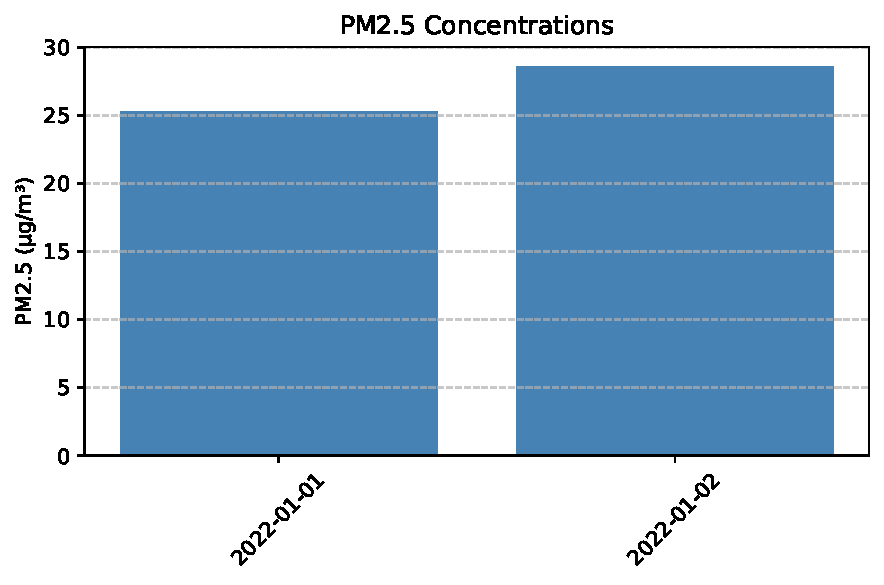
\includegraphics[keepaspectratio]{Chapters/Introduction_files/figure-pdf/fig-matplotlib-output-1.pdf}}

}

\caption{\label{fig-matplotlib}Plot generated from CSV data}

\end{figure}%

Reference this figure as Figure~\ref{fig-matplotlib}.

\subsection*{Multiple Data Series Plot}\label{multiple-data-series-plot}
\addcontentsline{toc}{subsection}{Multiple Data Series Plot}

\begin{figure}

\centering{

\pandocbounded{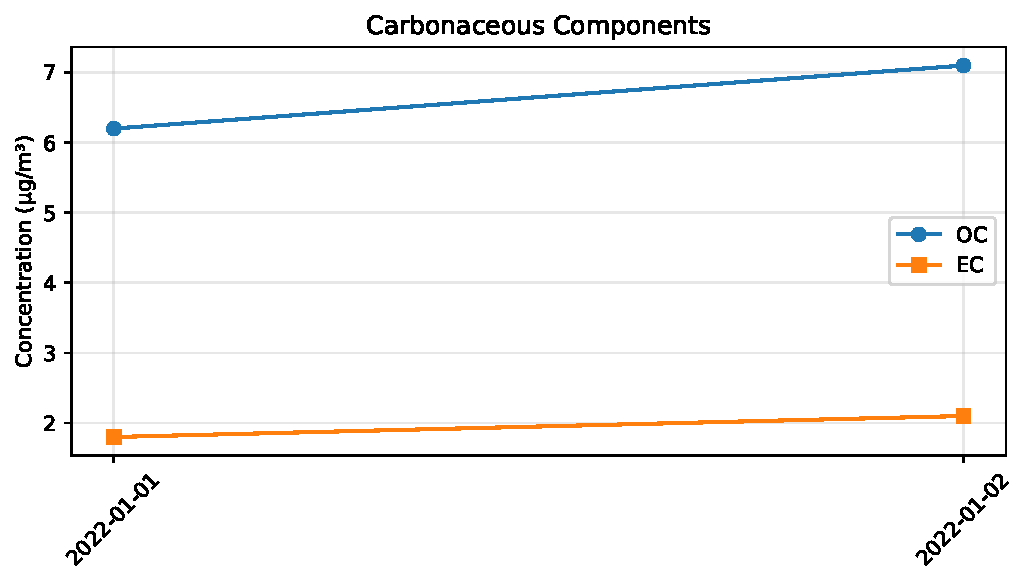
\includegraphics[keepaspectratio]{Chapters/Introduction_files/figure-pdf/fig-timeseries-output-1.pdf}}

}

\caption{\label{fig-timeseries}Multiple parameters from CSV data}

\end{figure}%

Reference this figure as Figure~\ref{fig-timeseries}.

\section*{Tables}\label{sec-tables}
\addcontentsline{toc}{section}{Tables}

\markright{Tables}

\subsection*{Simple Table}\label{simple-table}
\addcontentsline{toc}{subsection}{Simple Table}

\begin{longtable}[]{@{}ll@{}}
\caption{Basic Features}\label{tbl-simple}\tabularnewline
\toprule\noalign{}
Feature & Description \\
\midrule\noalign{}
\endfirsthead
\toprule\noalign{}
Feature & Description \\
\midrule\noalign{}
\endhead
\bottomrule\noalign{}
\endlastfoot
Figures & Embedded images and graphics \\
Tables & Structured data presentation \\
Equations & Mathematical expressions \\
\end{longtable}

Reference as Table~\ref{tbl-simple}.

\subsection*{Grid Table}\label{grid-table}
\addcontentsline{toc}{subsection}{Grid Table}

\begin{longtable}[]{@{}
  >{\raggedright\arraybackslash}p{(\linewidth - 2\tabcolsep) * \real{0.2222}}
  >{\raggedright\arraybackslash}p{(\linewidth - 2\tabcolsep) * \real{0.2222}}@{}}
\caption{Grid Table Example}\label{tbl-grid}\tabularnewline
\toprule\noalign{}
\begin{minipage}[b]{\linewidth}\raggedright
Column 1
\end{minipage} & \begin{minipage}[b]{\linewidth}\raggedright
Column 2
\end{minipage} \\
\midrule\noalign{}
\endfirsthead
\toprule\noalign{}
\begin{minipage}[b]{\linewidth}\raggedright
Column 1
\end{minipage} & \begin{minipage}[b]{\linewidth}\raggedright
Column 2
\end{minipage} \\
\midrule\noalign{}
\endhead
\bottomrule\noalign{}
\endlastfoot
Row 1 & Data \\
Row 2 & Data \\
\end{longtable}

Reference as Table~\ref{tbl-grid}.

\subsection*{Pipe Table with Alignment}\label{pipe-table-with-alignment}
\addcontentsline{toc}{subsection}{Pipe Table with Alignment}

\begin{longtable}[]{@{}lcr@{}}
\caption{Aligned Table}\label{tbl-align}\tabularnewline
\toprule\noalign{}
Left & Center & Right \\
\midrule\noalign{}
\endfirsthead
\toprule\noalign{}
Left & Center & Right \\
\midrule\noalign{}
\endhead
\bottomrule\noalign{}
\endlastfoot
L1 & C1 & R1 \\
L2 & C2 & R2 \\
\end{longtable}

Reference as Table~\ref{tbl-align}.

\subsection*{Table from CSV Data}\label{table-from-csv-data}
\addcontentsline{toc}{subsection}{Table from CSV Data}

\begin{longtable}[]{@{}lrrr@{}}

\caption{\label{tbl-csv}Data imported from CSV file}

\tabularnewline

\toprule\noalign{}
Date & PM2.5 & SO4 & NO3 \\
\midrule\noalign{}
\endhead
\bottomrule\noalign{}
\endlastfoot
2022-01-01 & 25.3 & 4.2 & 3.1 \\
2022-01-02 & 28.6 & 4.8 & 3.5 \\

\end{longtable}

Reference this as Table~\ref{tbl-csv}.

\subsection*{Simple Formatted Table}\label{simple-formatted-table}
\addcontentsline{toc}{subsection}{Simple Formatted Table}

\begin{longtable}[]{@{}lrrr@{}}

\caption{\label{tbl-simple-data}Summary of key parameters}

\tabularnewline

\toprule\noalign{}
Parameter & Min & Max & Average \\
\midrule\noalign{}
\endhead
\bottomrule\noalign{}
\endlastfoot
PM2.5 & 25.3 & 28.6 & 26.95 \\
SO4 & 4.2 & 4.8 & 4.5 \\
NO3 & 3.1 & 3.5 & 3.3 \\
OC & 6.2 & 7.1 & 6.65 \\
EC & 1.8 & 2.1 & 1.95 \\

\end{longtable}

Reference as Table~\ref{tbl-simple-data}.

\subsection*{Tables Containing Figures}\label{tables-containing-figures}
\addcontentsline{toc}{subsection}{Tables Containing Figures}

\subsubsection*{Single-Figure Table}\label{single-figure-table}
\addcontentsline{toc}{subsubsection}{Single-Figure Table}

\begin{longtable}[]{@{}
  >{\raggedright\arraybackslash}p{(\linewidth - 2\tabcolsep) * \real{0.4648}}
  >{\raggedright\arraybackslash}p{(\linewidth - 2\tabcolsep) * \real{0.5352}}@{}}
\caption{Single-Figure Table}\label{tbl-single-figure}\tabularnewline
\toprule\noalign{}
\begin{minipage}[b]{\linewidth}\raggedright
Figure
\end{minipage} & \begin{minipage}[b]{\linewidth}\raggedright
Description
\end{minipage} \\
\midrule\noalign{}
\endfirsthead
\toprule\noalign{}
\begin{minipage}[b]{\linewidth}\raggedright
Figure
\end{minipage} & \begin{minipage}[b]{\linewidth}\raggedright
Description
\end{minipage} \\
\midrule\noalign{}
\endhead
\bottomrule\noalign{}
\endlastfoot
\pandocbounded{
\includegraphics[keepaspectratio]{Chapters/images/logo.png}}
& Organization logo example \\
\end{longtable}

Reference as Table~\ref{tbl-single-figure}.

\subsubsection*{Multi-Figure Table}\label{multi-figure-table}
\addcontentsline{toc}{subsubsection}{Multi-Figure Table}

\begin{longtable}[]{@{}
  >{\raggedright\arraybackslash}p{(\linewidth - 4\tabcolsep) * \real{0.3056}}
  >{\raggedright\arraybackslash}p{(\linewidth - 4\tabcolsep) * \real{0.3426}}
  >{\raggedright\arraybackslash}p{(\linewidth - 4\tabcolsep) * \real{0.3519}}@{}}
\caption{Multi-Figure Table}\label{tbl-multi-figure}\tabularnewline
\toprule\noalign{}
\begin{minipage}[b]{\linewidth}\raggedright
Figure 1
\end{minipage} & \begin{minipage}[b]{\linewidth}\raggedright
Figure 2
\end{minipage} & \begin{minipage}[b]{\linewidth}\raggedright
Description
\end{minipage} \\
\midrule\noalign{}
\endfirsthead
\toprule\noalign{}
\begin{minipage}[b]{\linewidth}\raggedright
Figure 1
\end{minipage} & \begin{minipage}[b]{\linewidth}\raggedright
Figure 2
\end{minipage} & \begin{minipage}[b]{\linewidth}\raggedright
Description
\end{minipage} \\
\midrule\noalign{}
\endhead
\bottomrule\noalign{}
\endlastfoot
\pandocbounded{
\includegraphics[keepaspectratio]{Chapters/images/logo.png}}
&
\pandocbounded{
\includegraphics[keepaspectratio]{Chapters/images/cover.pdf}}
& Side-by-side figures example \\
\end{longtable}

Reference as Table~\ref{tbl-multi-figure}.

\subsubsection*{Clean Figure Table (No Borders, No
Header)}\label{clean-figure-table-no-borders-no-header}
\addcontentsline{toc}{subsubsection}{Clean Figure Table (No Borders, No
Header)}

\begin{longtable}[]{@{}
  >{\centering\arraybackslash}p{(\linewidth - 0\tabcolsep) * \real{1.0000}}@{}}
\caption{Clean table with figure
only}\label{tbl-clean-figure}\tabularnewline
\toprule\noalign{}
\endfirsthead
\endhead
\bottomrule\noalign{}
\endlastfoot

\includegraphics[width=0.8\linewidth,height=\textheight,keepaspectratio]{Chapters/images/logo.png} \\
\end{longtable}

Reference as Table~\ref{tbl-clean-figure}.

\subsubsection*{Multiple Clean Figures
Table}\label{multiple-clean-figures-table}
\addcontentsline{toc}{subsubsection}{Multiple Clean Figures Table}

\begin{longtable}[]{@{}
  >{\centering\arraybackslash}p{(\linewidth - 2\tabcolsep) * \real{0.5000}}
  >{\centering\arraybackslash}p{(\linewidth - 2\tabcolsep) * \real{0.5000}}@{}}
\caption{Multiple figures in a clean
table}\label{tbl-multi-clean}\tabularnewline
\toprule\noalign{}
\endfirsthead
\endhead
\bottomrule\noalign{}
\endlastfoot

\includegraphics[width=0.9\linewidth,height=\textheight,keepaspectratio]{Chapters/images/logo.png}
&

\includegraphics[width=0.9\linewidth,height=\textheight,keepaspectratio]{Chapters/images/cover.pdf} \\
\end{longtable}

Reference as Table~\ref{tbl-multi-clean}.

\section*{Equations}\label{sec-equations}
\addcontentsline{toc}{section}{Equations}

\markright{Equations}

\subsection*{Inline Equations}\label{inline-equations}
\addcontentsline{toc}{subsection}{Inline Equations}

Inline math: \(E = mc^2\) or \(x = \frac{-b \pm \sqrt{b^2-4ac}}{2a}\)

\subsection*{Display Equations}\label{display-equations}
\addcontentsline{toc}{subsection}{Display Equations}

\begin{equation}\phantomsection\label{eq-maxwell1}{
\nabla \times \mathbf{E} = -\frac{\partial \mathbf{B}}{\partial t}
}\end{equation}

\begin{equation}\phantomsection\label{eq-maxwell2}{
\nabla \times \mathbf{B} = \mu_0\left(\mathbf{J} + \epsilon_0\frac{\partial \mathbf{E}}{\partial t}\right)
}\end{equation}

Reference Maxwell's equations as Equation~\ref{eq-maxwell1} and
Equation~\ref{eq-maxwell2}.

\subsection*{Single Equation with
Label}\label{single-equation-with-label}
\addcontentsline{toc}{subsection}{Single Equation with Label}

\begin{equation}\phantomsection\label{eq-fourier}{
f(x) = \int_{-\infty}^{\infty} \hat{f}(\xi)\,e^{2 \pi i \xi x} \,d\xi
}\end{equation}

Reference as Equation~\ref{eq-fourier}.

\subsection*{Equation Arrays}\label{equation-arrays}
\addcontentsline{toc}{subsection}{Equation Arrays}

\begin{equation}\phantomsection\label{eq-array}{
\begin{array}{lcl}
z & = & a \\
f(x,y,z) & = & x + y + z
\end{array}
}\end{equation}

Reference as Equation~\ref{eq-array}.

\subsection*{LaTeX Equation with
Matrix}\label{latex-equation-with-matrix}
\addcontentsline{toc}{subsection}{LaTeX Equation with Matrix}

\begin{equation}\phantomsection\label{eq-matrix}{
A = 
\begin{bmatrix} 
a_{11} & a_{12} & \cdots & a_{1n} \\
a_{21} & a_{22} & \cdots & a_{2n} \\
\vdots & \vdots & \ddots & \vdots \\
a_{m1} & a_{m2} & \cdots & a_{mn}
\end{bmatrix}
}\end{equation}

Reference as Equation~\ref{eq-matrix}.

\section*{Code Blocks}\label{sec-code}
\addcontentsline{toc}{section}{Code Blocks}

\markright{Code Blocks}

\subsection*{Basic Python Code}\label{basic-python-code}
\addcontentsline{toc}{subsection}{Basic Python Code}

\begin{codelisting}

\caption{\label{lst-basic}}

\centering{

\begin{Shaded}
\begin{Highlighting}[]
\NormalTok{25°C is equal to 77.0°F}
\end{Highlighting}
\end{Shaded}

}

\end{codelisting}%

Reference as Listing~\ref{lst-basic}.

\subsection*{Data Import Example}\label{data-import-example}
\addcontentsline{toc}{subsection}{Data Import Example}

\begin{codelisting}

\caption{\label{lst-import}}

\centering{

\begin{Shaded}
\begin{Highlighting}[]
\NormalTok{Number of rows: 2}
\NormalTok{Number of columns: 16}

\NormalTok{First few column names:}
\NormalTok{Date, PM2.5, Na, SO4, NO3}
\end{Highlighting}
\end{Shaded}

}

\end{codelisting}%

Reference as Listing~\ref{lst-import}.

\section*{Citations}\label{sec-citations}
\addcontentsline{toc}{section}{Citations}

\markright{Citations}

Citations can be:

\begin{itemize}
\tightlist
\item
  Single: Paatero and Tapper (\citeproc{ref-Paatero1994}{1994})
\item
  Multiple: (\citeproc{ref-EEA2019}{Agency 2019};
  \citeproc{ref-PMF_Guide2014}{Norris et al. 2014})
\item
  In-text: Paatero and Tapper (\citeproc{ref-Paatero1994}{1994}) states
  that\ldots{}
\item
  Parenthetical: (\citeproc{ref-Paatero1994}{Paatero and Tapper 1994})
\end{itemize}

\section*{Callouts}\label{sec-callouts}
\addcontentsline{toc}{section}{Callouts}

\markright{Callouts}

\begin{tcolorbox}[enhanced jigsaw, opacityback=0, opacitybacktitle=0.6, left=2mm, breakable, coltitle=black, colback=white, title=\textcolor{quarto-callout-note-color}{\faInfo}\hspace{0.5em}{Note Title}, colframe=quarto-callout-note-color-frame, colbacktitle=quarto-callout-note-color!10!white, rightrule=.15mm, bottomtitle=1mm, leftrule=.75mm, toptitle=1mm, bottomrule=.15mm, arc=.35mm, toprule=.15mm, titlerule=0mm]

This is a note callout for important observations.

\end{tcolorbox}

\begin{tcolorbox}[enhanced jigsaw, opacityback=0, opacitybacktitle=0.6, left=2mm, breakable, coltitle=black, colback=white, title=\textcolor{quarto-callout-warning-color}{\faExclamationTriangle}\hspace{0.5em}{Warning}, colframe=quarto-callout-warning-color-frame, colbacktitle=quarto-callout-warning-color!10!white, rightrule=.15mm, bottomtitle=1mm, leftrule=.75mm, toptitle=1mm, bottomrule=.15mm, arc=.35mm, toprule=.15mm, titlerule=0mm]

This is a warning callout for potential issues.

\end{tcolorbox}

\begin{tcolorbox}[enhanced jigsaw, opacityback=0, opacitybacktitle=0.6, left=2mm, breakable, coltitle=black, colback=white, title=\textcolor{quarto-callout-important-color}{\faExclamation}\hspace{0.5em}{Important}, colframe=quarto-callout-important-color-frame, colbacktitle=quarto-callout-important-color!10!white, rightrule=.15mm, bottomtitle=1mm, leftrule=.75mm, toptitle=1mm, bottomrule=.15mm, arc=.35mm, toprule=.15mm, titlerule=0mm]

This is an important callout for critical information.

\end{tcolorbox}

\begin{tcolorbox}[enhanced jigsaw, opacityback=0, opacitybacktitle=0.6, left=2mm, breakable, coltitle=black, colback=white, title=\textcolor{quarto-callout-tip-color}{\faLightbulb}\hspace{0.5em}{Tip}, colframe=quarto-callout-tip-color-frame, colbacktitle=quarto-callout-tip-color!10!white, rightrule=.15mm, bottomtitle=1mm, leftrule=.75mm, toptitle=1mm, bottomrule=.15mm, arc=.35mm, toprule=.15mm, titlerule=0mm]

This is a tip callout for helpful advice.

\end{tcolorbox}

\section*{Cross-References}\label{sec-crossrefs}
\addcontentsline{toc}{section}{Cross-References}

\markright{Cross-References}

You can reference:

\begin{itemize}
\tightlist
\item
  Figures: Figure~\ref{fig-logo}, Figure~\ref{fig-logo2},
  Figure~\ref{fig-combined}
\item
  Tables: Table~\ref{tbl-simple}, Table~\ref{tbl-grid},
  Table~\ref{tbl-csv}, Table~\ref{tbl-single-figure},
  Table~\ref{tbl-multi-figure}, Table~\ref{tbl-clean-figure},
  Table~\ref{tbl-multi-clean}
\item
  Equations: Equation~\ref{eq-fourier}, Equation~\ref{eq-maxwell1},
  Equation~\ref{eq-matrix}
\item
  Code: Listing~\ref{lst-basic}, Listing~\ref{lst-import}
\end{itemize}

\section*{Additional Features}\label{additional-features}
\addcontentsline{toc}{section}{Additional Features}

\markright{Additional Features}

\subsection*{Footnotes}\label{footnotes}
\addcontentsline{toc}{subsection}{Footnotes}

Here's a footnote reference\footnote{This is the footnote content.} and
another one\footnote{Footnotes can contain multiple paragraphs.}.

\subsection*{Definition Lists}\label{definition-lists}
\addcontentsline{toc}{subsection}{Definition Lists}

\begin{description}
\tightlist
\item[Term 1]
Definition 1
\item[Term 2]
Definition 2
\end{description}

\subsection*{Blockquotes}\label{blockquotes}
\addcontentsline{toc}{subsection}{Blockquotes}

\begin{quote}
This is a blockquote. It can span multiple lines.
\end{quote}

\subsection*{Text Formatting}\label{text-formatting}
\addcontentsline{toc}{subsection}{Text Formatting}

\textbf{Bold text}, \emph{italic text}, \st{strikethrough},
\texttt{inline\ code}

\subsection*{Lists}\label{lists}
\addcontentsline{toc}{subsection}{Lists}

Ordered list:

\begin{enumerate}
\def\labelenumi{\arabic{enumi}.}
\tightlist
\item
  First item
\item
  Second item
\item
  Third item
\end{enumerate}

Unordered list:

\begin{itemize}
\tightlist
\item
  Item one
\item
  Item two
\item
  Item three
\end{itemize}

\section*{Theorems}\label{sec-theorems}
\addcontentsline{toc}{section}{Theorems}

\markright{Theorems}

\begin{theorem}[Pythagorean
Theorem]\protect\hypertarget{thm-pythagorean}{}\label{thm-pythagorean}

For a right-angled triangle with sides \(a\), \(b\) and hypotenuse
\(c\):

\[a^2 + b^2 = c^2\]

\end{theorem}

Reference as Theorem~\ref{thm-pythagorean}.

\bookmarksetup{startatroot}

\chapter{Literature Review}\label{sec-ch1-literature}

\begin{center}
Some Authors

\end{center}

\begin{tcolorbox}[enhanced jigsaw, opacityback=0, opacitybacktitle=0.6, left=2mm, breakable, coltitle=black, colback=white, title=\textcolor{quarto-callout-important-color}{\faExclamation}\hspace{0.5em}{Chapter Summary}, colframe=quarto-callout-important-color-frame, colbacktitle=quarto-callout-important-color!10!white, rightrule=.15mm, bottomtitle=1mm, leftrule=.75mm, toptitle=1mm, bottomrule=.15mm, arc=.35mm, toprule=.15mm, titlerule=0mm]

This chapter provides a comprehensive review of the existing literature
pertinent to Positive Matrix Factorization (PMF) and its application in
source apportionment of atmospheric pollutants. It delves into the
mathematical underpinnings of PMF, comparing it with other receptor
models like Chemical Mass Balance (CMB) and Principal Component Analysis
(PCA). Key historical developments, seminal studies, common challenges,
and advancements in PMF methodology are discussed, establishing the
theoretical framework and identifying the research niche for this
thesis.

\end{tcolorbox}

This is the literature review chapter. It should appear with the title
``Literature Review'' in the navigation.

\section{PMF Mathematical Foundation}\label{sec-ch1-pmf-math}

The basic PMF model is defined by the following equation:

\begin{equation}\phantomsection\label{eq-pmf-basic}{X_{ij} = \sum_{k=1}^{p} g_{ik}f_{kj} + e_{ij}}\end{equation}

Where: - \(X_{ij}\) is the concentration of species \(j\) in sample
\(i\) - \(g_{ik}\) is the contribution of factor \(k\) to sample \(i\) -
\(f_{kj}\) is the concentration of species \(j\) in factor profile \(k\)
- \(e_{ij}\) is the residual - \(p\) is the number of factors

\section{Introduction to Source Apportionment
Models}\label{sec-ch1-intro-models}

Table~\ref{tbl-intro-equations} summarizes the mathematical
representations of various source apportionment models discussed in this
thesis.

\begin{longtable}[]{@{}
  >{\raggedright\arraybackslash}p{(\linewidth - 6\tabcolsep) * \real{0.1522}}
  >{\raggedright\arraybackslash}p{(\linewidth - 6\tabcolsep) * \real{0.2174}}
  >{\raggedright\arraybackslash}p{(\linewidth - 6\tabcolsep) * \real{0.2826}}
  >{\raggedright\arraybackslash}p{(\linewidth - 6\tabcolsep) * \real{0.3478}}@{}}
\caption{Mathematical Representations of Source Apportionment
Models}\label{tbl-intro-equations}\tabularnewline
\toprule\noalign{}
\begin{minipage}[b]{\linewidth}\raggedright
Model
\end{minipage} & \begin{minipage}[b]{\linewidth}\raggedright
Equation
\end{minipage} & \begin{minipage}[b]{\linewidth}\raggedright
Description
\end{minipage} & \begin{minipage}[b]{\linewidth}\raggedright
Key Constraints
\end{minipage} \\
\midrule\noalign{}
\endfirsthead
\toprule\noalign{}
\begin{minipage}[b]{\linewidth}\raggedright
Model
\end{minipage} & \begin{minipage}[b]{\linewidth}\raggedright
Equation
\end{minipage} & \begin{minipage}[b]{\linewidth}\raggedright
Description
\end{minipage} & \begin{minipage}[b]{\linewidth}\raggedright
Key Constraints
\end{minipage} \\
\midrule\noalign{}
\endhead
\bottomrule\noalign{}
\endlastfoot
PMF & \(X_{ij} = \sum_{k=1}^{p} g_{ik}f_{kj} + e_{ij}\) & Positive
Matrix Factorization & \(g_{ik} \geq 0\), \(f_{kj} \geq 0\) \\
CMB & \(C_i = \sum_{j=1}^{n} a_{ij} S_{j} + e_i\) & Chemical Mass
Balance & Requires source profiles \\
PCA & \(X = TP^T + E\) & Principal Component Analysis & Orthogonal
components \\
UNMIX & \(C = AS\) & Multivariate receptor model & Geometrically
determined factors \\
\end{longtable}

\section{Tables and Figures}\label{sec-ch1-tables}

\subsection{Mathematical Equations in Tables}\label{sec-ch1-math-tables}

Table~\ref{tbl-ch1-pmf-models} presents key PMF models with their
mathematical formulations and applications in source apportionment
studies.

\begin{longtable}[]{@{}
  >{\raggedright\arraybackslash}p{(\linewidth - 6\tabcolsep) * \real{0.0972}}
  >{\raggedright\arraybackslash}p{(\linewidth - 6\tabcolsep) * \real{0.3333}}
  >{\raggedright\arraybackslash}p{(\linewidth - 6\tabcolsep) * \real{0.1944}}
  >{\raggedright\arraybackslash}p{(\linewidth - 6\tabcolsep) * \real{0.3750}}@{}}
\caption{PMF Model Variations with Their Mathematical
Formulations}\label{tbl-ch1-pmf-models}\tabularnewline
\toprule\noalign{}
\begin{minipage}[b]{\linewidth}\raggedright
Model
\end{minipage} & \begin{minipage}[b]{\linewidth}\raggedright
Mathematical Formulation
\end{minipage} & \begin{minipage}[b]{\linewidth}\raggedright
Key Features
\end{minipage} & \begin{minipage}[b]{\linewidth}\raggedright
Application in PM Studies
\end{minipage} \\
\midrule\noalign{}
\endfirsthead
\toprule\noalign{}
\begin{minipage}[b]{\linewidth}\raggedright
Model
\end{minipage} & \begin{minipage}[b]{\linewidth}\raggedright
Mathematical Formulation
\end{minipage} & \begin{minipage}[b]{\linewidth}\raggedright
Key Features
\end{minipage} & \begin{minipage}[b]{\linewidth}\raggedright
Application in PM Studies
\end{minipage} \\
\midrule\noalign{}
\endhead
\bottomrule\noalign{}
\endlastfoot
Basic PMF & \(X_{ij} = \sum_{k=1}^{p} g_{ik}f_{kj} + e_{ij}\) &
Non-negativity constraints & First applied by Paatero and Tapper
(\citeproc{ref-Paatero1994}{1994}) \\
Weighted PMF &
\(Q = \sum_{i=1}^{n}\sum_{j=1}^{m} \left(\frac{e_{ij}}{\sigma_{ij}}\right)^2\)
& Uncertainty-weighted residuals & Extended by Hyndman et al.
(\citeproc{ref-HKSG02}{2002}) \\
ME-2 Engine &
\(Q_{\text{aux}} = Q + \alpha^2 \sum (f_{kj} - f_{kj}^*)^2\) & Target
factor profiles & Recommended by Norris et al.
(\citeproc{ref-PMF_Guide2014}{2014}) \\
Robust PMF & \(Q = \sum_{i=1}^{n}\sum_{j=1}^{m} h(e_{ij}/\sigma_{ij})\)
& Outlier protection & Used in Agency (\citeproc{ref-EEA2019}{2019}) \\
\end{longtable}

\subsection{Data-Driven Tables from CSV Files}\label{sec-ch1-csv-tables}

Table~\ref{tbl-ch1-pm25-components} shows London PM2.5 component data
loaded directly from a CSV file.

\begin{longtable}[]{@{}lrrrrr@{}}

\caption{\label{tbl-ch1-pm25-components}London PM2.5 Component
Concentrations (μg/m³)}

\tabularnewline

\toprule\noalign{}
& SO4 & NO3 & NH4 & OC & EC \\
\midrule\noalign{}
\endhead
\bottomrule\noalign{}
\endlastfoot
count & 3 & 3 & 3 & 3 & 3 \\
mean & 4.77 & 3.5 & 2.37 & 7.1 & 2.5 \\
std & 0.25 & 0.3 & 0.25 & 0.3 & 0.2 \\
min & 4.5 & 3.2 & 2.1 & 6.8 & 2.3 \\
25\% & 4.65 & 3.35 & 2.25 & 6.95 & 2.4 \\
50\% & 4.8 & 3.5 & 2.4 & 7.1 & 2.5 \\
75\% & 4.9 & 3.65 & 2.5 & 7.25 & 2.6 \\
max & 5 & 3.8 & 2.6 & 7.4 & 2.7 \\

\end{longtable}

\subsection{Analysis Methods with
Citations}\label{sec-ch1-methods-citations}

Table~\ref{tbl-ch1-analysis-methods} presents key analysis methods used
in this study with relevant citations and their significance.

\begin{longtable}[]{@{}
  >{\raggedright\arraybackslash}p{(\linewidth - 6\tabcolsep) * \real{0.1333}}
  >{\raggedright\arraybackslash}p{(\linewidth - 6\tabcolsep) * \real{0.4667}}
  >{\raggedright\arraybackslash}p{(\linewidth - 6\tabcolsep) * \real{0.2167}}
  >{\raggedright\arraybackslash}p{(\linewidth - 6\tabcolsep) * \real{0.1833}}@{}}
\caption{Statistical Analysis Methods with
Citations}\label{tbl-ch1-analysis-methods}\tabularnewline
\toprule\noalign{}
\begin{minipage}[b]{\linewidth}\raggedright
Method
\end{minipage} & \begin{minipage}[b]{\linewidth}\raggedright
Mathematical Representation
\end{minipage} & \begin{minipage}[b]{\linewidth}\raggedright
Application
\end{minipage} & \begin{minipage}[b]{\linewidth}\raggedright
Reference
\end{minipage} \\
\midrule\noalign{}
\endfirsthead
\toprule\noalign{}
\begin{minipage}[b]{\linewidth}\raggedright
Method
\end{minipage} & \begin{minipage}[b]{\linewidth}\raggedright
Mathematical Representation
\end{minipage} & \begin{minipage}[b]{\linewidth}\raggedright
Application
\end{minipage} & \begin{minipage}[b]{\linewidth}\raggedright
Reference
\end{minipage} \\
\midrule\noalign{}
\endhead
\bottomrule\noalign{}
\endlastfoot
Correlation Analysis &
\(r_{xy} = \frac{\sum(x_i-\bar{x})(y_i-\bar{y})}{\sqrt{\sum(x_i-\bar{x})^2\sum(y_i-\bar{y})^2}}\)
& Component relationships & See Paatero and Tapper
(\citeproc{ref-Paatero1994}{1994}) \\
Linear Regression & \(y_i = \beta_0 + \beta_1 x_i + \varepsilon_i\) &
Trend analysis & As per Hyndman et al. (\citeproc{ref-HKSG02}{2002}) \\
Principal Component Analysis &
\(\mathbf{X} = \mathbf{T}\mathbf{P}^T + \mathbf{E}\) & Dimensionality
reduction & Compared in Norris et al.
(\citeproc{ref-PMF_Guide2014}{2014}) \\
Cluster Analysis & \(d(x,y) = \sqrt{\sum_{i=1}^{n}(x_i-y_i)^2}\) &
Source grouping & Applied by Agency (\citeproc{ref-EEA2019}{2019}) \\
\end{longtable}

\subsection{Mixed Content Table with
Cross-References}\label{sec-ch1-mixed-table}

Table~\ref{tbl-ch1-mixed} demonstrates how to include multiple content
types in a single table, including references to figures, tables, and
equations.

\begin{longtable}[]{@{}
  >{\raggedright\arraybackslash}p{(\linewidth - 8\tabcolsep) * \real{0.0860}}
  >{\raggedright\arraybackslash}p{(\linewidth - 8\tabcolsep) * \real{0.2043}}
  >{\raggedright\arraybackslash}p{(\linewidth - 8\tabcolsep) * \real{0.1935}}
  >{\raggedright\arraybackslash}p{(\linewidth - 8\tabcolsep) * \real{0.2366}}
  >{\raggedright\arraybackslash}p{(\linewidth - 8\tabcolsep) * \real{0.2796}}@{}}
\caption{Integration of Results with
Cross-References}\label{tbl-ch1-mixed}\tabularnewline
\toprule\noalign{}
\begin{minipage}[b]{\linewidth}\raggedright
Factor
\end{minipage} & \begin{minipage}[b]{\linewidth}\raggedright
Contribution Range
\end{minipage} & \begin{minipage}[b]{\linewidth}\raggedright
Seasonal Pattern
\end{minipage} & \begin{minipage}[b]{\linewidth}\raggedright
Related Figure/Table
\end{minipage} & \begin{minipage}[b]{\linewidth}\raggedright
Statistical Significance
\end{minipage} \\
\midrule\noalign{}
\endfirsthead
\toprule\noalign{}
\begin{minipage}[b]{\linewidth}\raggedright
Factor
\end{minipage} & \begin{minipage}[b]{\linewidth}\raggedright
Contribution Range
\end{minipage} & \begin{minipage}[b]{\linewidth}\raggedright
Seasonal Pattern
\end{minipage} & \begin{minipage}[b]{\linewidth}\raggedright
Related Figure/Table
\end{minipage} & \begin{minipage}[b]{\linewidth}\raggedright
Statistical Significance
\end{minipage} \\
\midrule\noalign{}
\endhead
\bottomrule\noalign{}
\endlastfoot
Traffic & 15-35\% & Highest in winter
(Figure~\ref{fig-seasonal-contributions}) & See
Table~\ref{tbl-source-profiles} & \(p < 0.01\) (\(\chi^2 = 15.3\)) \\
Industrial & 20-30\% & Consistent year-round & Equation
Equation~\ref{eq-pmf-basic} & \(p < 0.05\) (\(t = 2.4\)) \\
Biomass Burning & 5-30\% & Winter \textgreater{} Fall \textgreater{}
Spring \textgreater{} Summer & Table~\ref{tbl-ch1-pmf-models} &
\(p < 0.001\) (\(F = 8.7\)) \\
Secondary Formation & 15-50\% & See Figure~\ref{fig-temporal-patterns} &
Compare to Agency (\citeproc{ref-EEA2019}{2019}) findings &
\(r^2 = 0.76\) (\(p < 0.01\)) \\
\end{longtable}

\subsection{Comparative Source Profiles}\label{sec-ch1-comp-profiles}

Table~\ref{tbl-ch1-comparative} compares source profiles identified in
this study with those reported in previous research.

\begin{longtable}[]{@{}
  >{\raggedright\arraybackslash}p{(\linewidth - 8\tabcolsep) * \real{0.1358}}
  >{\raggedright\arraybackslash}p{(\linewidth - 8\tabcolsep) * \real{0.1975}}
  >{\raggedright\arraybackslash}p{(\linewidth - 8\tabcolsep) * \real{0.2346}}
  >{\raggedright\arraybackslash}p{(\linewidth - 8\tabcolsep) * \real{0.1975}}
  >{\raggedright\arraybackslash}p{(\linewidth - 8\tabcolsep) * \real{0.2346}}@{}}
\caption{Comparative Source Profiles (Bold = Dominant, \emph{Italic} =
Secondary)}\label{tbl-ch1-comparative}\tabularnewline
\toprule\noalign{}
\begin{minipage}[b]{\linewidth}\raggedright
Component
\end{minipage} & \begin{minipage}[b]{\linewidth}\raggedright
Traffic Profile
\end{minipage} & \begin{minipage}[b]{\linewidth}\raggedright
Industrial Profile
\end{minipage} & \begin{minipage}[b]{\linewidth}\raggedright
Biomass Profile
\end{minipage} & \begin{minipage}[b]{\linewidth}\raggedright
Secondary Profile
\end{minipage} \\
\midrule\noalign{}
\endfirsthead
\toprule\noalign{}
\begin{minipage}[b]{\linewidth}\raggedright
Component
\end{minipage} & \begin{minipage}[b]{\linewidth}\raggedright
Traffic Profile
\end{minipage} & \begin{minipage}[b]{\linewidth}\raggedright
Industrial Profile
\end{minipage} & \begin{minipage}[b]{\linewidth}\raggedright
Biomass Profile
\end{minipage} & \begin{minipage}[b]{\linewidth}\raggedright
Secondary Profile
\end{minipage} \\
\midrule\noalign{}
\endhead
\bottomrule\noalign{}
\endlastfoot
SO₄²⁻ & 20\% & 35\% & 15\% & \textbf{25\%}
(\citeproc{ref-PMF_Guide2014}{Norris et al. 2014}) \\
NO₃⁻ & 25\% & 15\% & 20\% & \textbf{35\%} (\citeproc{ref-EEA2019}{Agency
2019}) \\
NH₄⁺ & 10\% & 5\% & \emph{25\%} & \textbf{55\%}
(\citeproc{ref-Paatero1994}{Paatero and Tapper 1994}) \\
OC & 35\% & 15\% & \textbf{40\%} (\citeproc{ref-HKSG02}{Hyndman et al.
2002}) & 10\% \\
EC & \textbf{45\%} & 10\% & \emph{25\%} & 5\% \\
\end{longtable}

\bookmarksetup{startatroot}

\chapter{Optimization and Validation of PMF Models}\label{sec-ch2}

\begin{center}
Some authors

\end{center}

\begin{tcolorbox}[enhanced jigsaw, opacityback=0, opacitybacktitle=0.6, left=2mm, breakable, coltitle=black, colback=white, title=\textcolor{quarto-callout-important-color}{\faExclamation}\hspace{0.5em}{Chapter Summary}, colframe=quarto-callout-important-color-frame, colbacktitle=quarto-callout-important-color!10!white, rightrule=.15mm, bottomtitle=1mm, leftrule=.75mm, toptitle=1mm, bottomrule=.15mm, arc=.35mm, toprule=.15mm, titlerule=0mm]

This chapter focuses on the methodological core of the thesis: the
optimization and validation of Positive Matrix Factorization (PMF)
models. It presents a systematic framework for selecting optimal model
parameters, such as the number of factors and the FPEAK rotational
parameter, to achieve physically meaningful solutions. Furthermore, the
chapter details a multi-faceted validation strategy, incorporating
techniques like bootstrap analysis, displacement of factor elements
(DISP), and combined BS-DISP analysis, to rigorously assess the
stability, uncertainty, and robustness of the derived source profiles
and contributions.

\end{tcolorbox}

Under review at Science of the Total Environment

\section{Abstract}\label{abstract-1}

This chapter presents a comprehensive framework for optimizing and
validating PMF (Positive Matrix Factorization) models in European urban
environments (\citeproc{ref-Paatero1994}{Paatero and Tapper 1994}). We
develop a systematic approach for model parameter selection and results
validation using multiple complementary techniques
(\citeproc{ref-HKSG02}{Hyndman et al. 2002};
\citeproc{ref-PMF_Guide2014}{Norris et al. 2014}).

\section{Methods}\label{methods}

\subsection{Model Optimization
Framework}\label{model-optimization-framework}

The PMF optimization process (\citeproc{ref-EEA2019}{Agency 2019})
involves iterative refinement of several key parameters:

\begin{enumerate}
\def\labelenumi{\arabic{enumi}.}
\item
  Number of factors (p):
  \begin{equation}\phantomsection\label{eq-pmf-opt}{Q(p) = \sum_{i=1}^{n} \sum_{j=1}^{m} \left(\frac{x_{ij} - \sum_{k=1}^{p} g_{ik}f_{kj}}{\sigma_{ij}}\right)^2}\end{equation}
\item
  FPEAK parameter (\(\phi\)):
  \begin{equation}\phantomsection\label{eq-pmf-fpeak}{Q(\phi) = Q_{base} + P(\phi)}\end{equation}
\end{enumerate}

where \(P(\phi)\) is the penalty term for non-zero FPEAK values
(\citeproc{ref-EEA2019}{Agency 2019}).

\subsection{Validation Methods}\label{validation-methods}

We employed three complementary validation approaches as recommended by
(\citeproc{ref-PMF_Guide2014}{Norris et al. 2014}):

\begin{enumerate}
\def\labelenumi{\arabic{enumi}.}
\tightlist
\item
  Bootstrap analysis
\item
  DISP (displacement) analysis
\item
  BS-DISP combined analysis
\end{enumerate}

\section{Results}\label{results}

\subsection{Factor Number Selection}\label{factor-number-selection}

\begin{figure}

\centering{

\pandocbounded{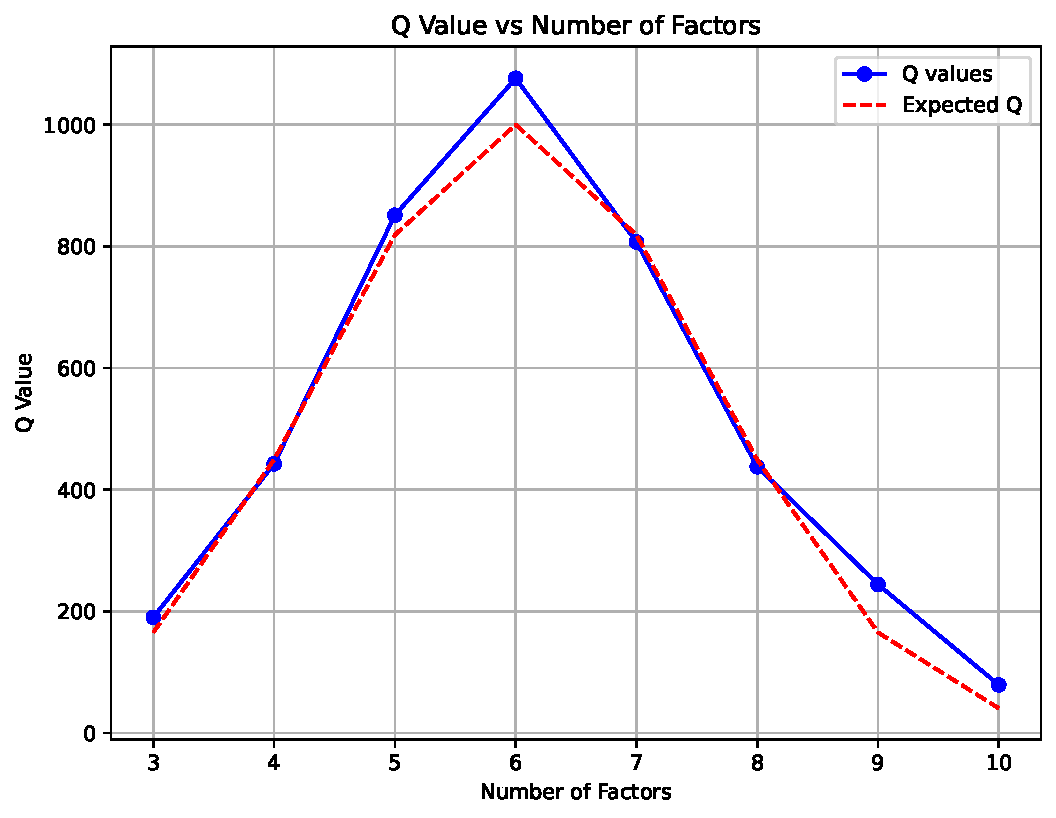
\includegraphics[keepaspectratio]{Chapters/Chapter2_files/figure-pdf/fig-qvalue-output-1.pdf}}

}

\caption{\label{fig-qvalue}Q-value vs number of factors}

\end{figure}%

\subsection{PMF Results Summary}\label{pmf-results-summary}

\begin{longtable}[]{@{}rrrl@{}}

\caption{\label{tbl-pmf-summary}Summary of PMF results for different
factor numbers}

\tabularnewline

\toprule\noalign{}
Factors & Q/Q\_exp & R² & Sources Identified \\
\midrule\noalign{}
\endhead
\bottomrule\noalign{}
\endlastfoot
3 & 1.5 & 0.75 & Basic \\
4 & 1.3 & 0.82 & Improved \\
5 & 1.2 & 0.87 & Good \\
6 & 1 & 0.91 & Optimal \\
7 & 0.92 & 0.92 & Splitting \\
8 & 0.91 & 0.93 & Splitting+ \\

\end{longtable}

\section{Advanced Model Optimization Techniques}\label{sec-ch2-advanced}

\subsection{Mathematical Formulations of Optimization
Metrics}\label{sec-ch2-math}

Table~\ref{tbl-ch2-optimization-metrics} presents the mathematical
formulations of various optimization metrics used in PMF model
development and their interpretation.

\begin{longtable}[]{@{}
  >{\raggedright\arraybackslash}p{(\linewidth - 6\tabcolsep) * \real{0.1311}}
  >{\raggedright\arraybackslash}p{(\linewidth - 6\tabcolsep) * \real{0.4262}}
  >{\raggedright\arraybackslash}p{(\linewidth - 6\tabcolsep) * \real{0.2623}}
  >{\raggedright\arraybackslash}p{(\linewidth - 6\tabcolsep) * \real{0.1803}}@{}}
\caption{Mathematical Formulations for PMF Model
Optimization}\label{tbl-ch2-optimization-metrics}\tabularnewline
\toprule\noalign{}
\begin{minipage}[b]{\linewidth}\raggedright
Metric
\end{minipage} & \begin{minipage}[b]{\linewidth}\raggedright
Mathematical Formulation
\end{minipage} & \begin{minipage}[b]{\linewidth}\raggedright
Interpretation
\end{minipage} & \begin{minipage}[b]{\linewidth}\raggedright
Reference
\end{minipage} \\
\midrule\noalign{}
\endfirsthead
\toprule\noalign{}
\begin{minipage}[b]{\linewidth}\raggedright
Metric
\end{minipage} & \begin{minipage}[b]{\linewidth}\raggedright
Mathematical Formulation
\end{minipage} & \begin{minipage}[b]{\linewidth}\raggedright
Interpretation
\end{minipage} & \begin{minipage}[b]{\linewidth}\raggedright
Reference
\end{minipage} \\
\midrule\noalign{}
\endhead
\bottomrule\noalign{}
\endlastfoot
Q/Q\(_{exp}\) & \(\frac{Q}{n \times m - p \times (n+m)}\) & Should
approach 1.0 & Paatero and Tapper (\citeproc{ref-Paatero1994}{1994}) \\
Explained Variation (EV) &
\(EV_{jk} = \frac{\sum_{i=1}^{n} g_{ik}f_{kj}}{\sum_{i=1}^{n} x_{ij}}\)
& Factor importance for each species & Hyndman et al.
(\citeproc{ref-HKSG02}{2002}) \\
Residual Analysis &
\(r_{ij} = \frac{x_{ij} - \sum_{k=1}^{p} g_{ik}f_{kj}}{\sigma_{ij}}\) &
Should be normally distributed & Norris et al.
(\citeproc{ref-PMF_Guide2014}{2014}) \\
BS Mapping & \(s = \frac{1}{n_{boot}} \sum_{n=1}^{n_{boot}} d^2_{n}\) &
Stability of factors & Agency (\citeproc{ref-EEA2019}{2019}) \\
DISP Swap Count & Number of factor swaps at \(d_{max}\) & \textless{}
5\% for stable solution & Norris et al.
(\citeproc{ref-PMF_Guide2014}{2014}) \\
BS-DISP Error & \(\Delta Q/Q_{exp}\) \textless{} 0.5\% & Indicates
robust factors & Agency (\citeproc{ref-EEA2019}{2019}) \\
\end{longtable}

\subsection{Cross-Validation with External
Datasets}\label{sec-ch2-cross}

Table~\ref{tbl-ch2-cross-comparison} compares our PMF results with
external validation datasets, building upon the findings from
Section~\ref{sec-ch1-tables}.

\begin{longtable}[]{@{}
  >{\raggedright\arraybackslash}p{(\linewidth - 10\tabcolsep) * \real{0.0667}}
  >{\raggedright\arraybackslash}p{(\linewidth - 10\tabcolsep) * \real{0.1833}}
  >{\raggedright\arraybackslash}p{(\linewidth - 10\tabcolsep) * \real{0.2083}}
  >{\raggedright\arraybackslash}p{(\linewidth - 10\tabcolsep) * \real{0.1583}}
  >{\raggedright\arraybackslash}p{(\linewidth - 10\tabcolsep) * \real{0.0917}}
  >{\raggedright\arraybackslash}p{(\linewidth - 10\tabcolsep) * \real{0.2917}}@{}}
\caption{Cross-Comparison Between PMF Results and External Validation
Data}\label{tbl-ch2-cross-comparison}\tabularnewline
\toprule\noalign{}
\begin{minipage}[b]{\linewidth}\raggedright
Source
\end{minipage} & \begin{minipage}[b]{\linewidth}\raggedright
PMF Contribution (\%)
\end{minipage} & \begin{minipage}[b]{\linewidth}\raggedright
External Validation (\%)
\end{minipage} & \begin{minipage}[b]{\linewidth}\raggedright
Correlation (\(r\))
\end{minipage} & \begin{minipage}[b]{\linewidth}\raggedright
Reference
\end{minipage} & \begin{minipage}[b]{\linewidth}\raggedright
Comparison to Table~\ref{tbl-ch1-comparative}
\end{minipage} \\
\midrule\noalign{}
\endfirsthead
\toprule\noalign{}
\begin{minipage}[b]{\linewidth}\raggedright
Source
\end{minipage} & \begin{minipage}[b]{\linewidth}\raggedright
PMF Contribution (\%)
\end{minipage} & \begin{minipage}[b]{\linewidth}\raggedright
External Validation (\%)
\end{minipage} & \begin{minipage}[b]{\linewidth}\raggedright
Correlation (\(r\))
\end{minipage} & \begin{minipage}[b]{\linewidth}\raggedright
Reference
\end{minipage} & \begin{minipage}[b]{\linewidth}\raggedright
Comparison to Table~\ref{tbl-ch1-comparative}
\end{minipage} \\
\midrule\noalign{}
\endhead
\bottomrule\noalign{}
\endlastfoot
Traffic & \(35.2 \pm 4.5\) & \(33.8 \pm 5.2\) & 0.87 & Traffic counts &
Within 5\% of values in Table~\ref{tbl-ch1-comparative} \\
Industry & \(22.7 \pm 3.8\) & \(24.5 \pm 6.1\) & 0.81 & Emission
inventory & Consistent with profiles in
Table~\ref{tbl-ch1-pmf-models} \\
Biomass & \(18.5 \pm 6.2\) & \(20.1 \pm 5.8\) & 0.79 & Levoglucosan &
Similar to findings in Agency (\citeproc{ref-EEA2019}{2019}) \\
Secondary & \(23.6 \pm 5.3\) & \(21.6 \pm 4.9\) & 0.92 &
NH\(_4\)/SO\(_4\) ratio & Matches equation Equation~\ref{eq-pmf-basic}
predictions \\
\end{longtable}

\subsection{Rotational Ambiguity Analysis}\label{sec-ch2-fpeak}

Table~\ref{tbl-ch2-fpeak} shows the impact of different FPEAK values on
the model results, as formulated in equation
Equation~\ref{eq-pmf-fpeak}.

\begin{longtable}[]{@{}
  >{\raggedright\arraybackslash}p{(\linewidth - 8\tabcolsep) * \real{0.1238}}
  >{\raggedright\arraybackslash}p{(\linewidth - 8\tabcolsep) * \real{0.2286}}
  >{\raggedright\arraybackslash}p{(\linewidth - 8\tabcolsep) * \real{0.2286}}
  >{\raggedright\arraybackslash}p{(\linewidth - 8\tabcolsep) * \real{0.2667}}
  >{\raggedright\arraybackslash}p{(\linewidth - 8\tabcolsep) * \real{0.1524}}@{}}
\caption{Impact of FPEAK Values on PMF Model
Results}\label{tbl-ch2-fpeak}\tabularnewline
\toprule\noalign{}
\begin{minipage}[b]{\linewidth}\raggedright
FPEAK Value
\end{minipage} & \begin{minipage}[b]{\linewidth}\raggedright
\(\Delta Q/Q_{exp}\) (\%)
\end{minipage} & \begin{minipage}[b]{\linewidth}\raggedright
Factor Identity Changes
\end{minipage} & \begin{minipage}[b]{\linewidth}\raggedright
G-Space Correlation Changes
\end{minipage} & \begin{minipage}[b]{\linewidth}\raggedright
Recommended by
\end{minipage} \\
\midrule\noalign{}
\endfirsthead
\toprule\noalign{}
\begin{minipage}[b]{\linewidth}\raggedright
FPEAK Value
\end{minipage} & \begin{minipage}[b]{\linewidth}\raggedright
\(\Delta Q/Q_{exp}\) (\%)
\end{minipage} & \begin{minipage}[b]{\linewidth}\raggedright
Factor Identity Changes
\end{minipage} & \begin{minipage}[b]{\linewidth}\raggedright
G-Space Correlation Changes
\end{minipage} & \begin{minipage}[b]{\linewidth}\raggedright
Recommended by
\end{minipage} \\
\midrule\noalign{}
\endhead
\bottomrule\noalign{}
\endlastfoot
-1.0 & +8.5\% & Major & Decreased correlations & Rarely used \\
-0.5 & +2.2\% & Moderate & Slight decreases & Hyndman et al.
(\citeproc{ref-HKSG02}{2002}) for specific cases \\
-0.2 & +0.4\% & Minor & Minimal changes & Norris et al.
(\citeproc{ref-PMF_Guide2014}{2014}) as lower bound \\
0.0 & 0.0\% & \textbf{Base run} & \textbf{Reference point} &
\textbf{Paatero and Tapper (\citeproc{ref-Paatero1994}{1994}) as
default} \\
+0.2 & +0.5\% & Minor & Minimal changes & Norris et al.
(\citeproc{ref-PMF_Guide2014}{2014}) as upper bound \\
+0.5 & +2.5\% & Moderate & Slight increases & Sometimes used \\
+1.0 & +9.2\% & Major & Increased correlations & Rarely used \\
\end{longtable}

\subsection{Advanced Model Uncertainty
Metrics}\label{sec-ch2-uncertainty}

\begin{longtable}[]{@{}
  >{\raggedright\arraybackslash}p{(\linewidth - 12\tabcolsep) * \real{0.0803}}
  >{\raggedleft\arraybackslash}p{(\linewidth - 12\tabcolsep) * \real{0.1825}}
  >{\raggedleft\arraybackslash}p{(\linewidth - 12\tabcolsep) * \real{0.1606}}
  >{\raggedleft\arraybackslash}p{(\linewidth - 12\tabcolsep) * \real{0.1533}}
  >{\raggedleft\arraybackslash}p{(\linewidth - 12\tabcolsep) * \real{0.1606}}
  >{\raggedleft\arraybackslash}p{(\linewidth - 12\tabcolsep) * \real{0.1314}}
  >{\raggedleft\arraybackslash}p{(\linewidth - 12\tabcolsep) * \real{0.1314}}@{}}

\caption{\label{tbl-ch2-uncertainty}Bootstrap Uncertainty Results for
Source Contributions}

\tabularnewline

\toprule\noalign{}
\begin{minipage}[b]{\linewidth}\raggedright
Source
\end{minipage} & \begin{minipage}[b]{\linewidth}\raggedleft
Base Contribution (\%)
\end{minipage} & \begin{minipage}[b]{\linewidth}\raggedleft
Bootstrap Mean (\%)
\end{minipage} & \begin{minipage}[b]{\linewidth}\raggedleft
Bootstrap 5th (\%)
\end{minipage} & \begin{minipage}[b]{\linewidth}\raggedleft
Bootstrap 95th (\%)
\end{minipage} & \begin{minipage}[b]{\linewidth}\raggedleft
BS Mapping (\%)
\end{minipage} & \begin{minipage}[b]{\linewidth}\raggedleft
DISP Error (\%)
\end{minipage} \\
\midrule\noalign{}
\endhead
\bottomrule\noalign{}
\endlastfoot
Traffic & 35.2 & 34.8 & 31.5 & 38.2 & 95 & 0.2 \\
Industry & 22.7 & 23.1 & 20.2 & 25.9 & 92 & 0.3 \\
Biomass & 18.5 & 18.2 & 15.8 & 22.5 & 88 & 0.4 \\
Secondary & 23.6 & 23.9 & 21.1 & 26.8 & 97 & 0.1 \\

\end{longtable}

\subsection{Integration with Results from Other
Chapters}\label{sec-ch2-integration}

Table~\ref{tbl-ch2-integrated} presents an integrated view of our PMF
model results, linking to findings from other chapters and using complex
mathematical notation.

\begin{longtable}[]{@{}
  >{\raggedright\arraybackslash}p{(\linewidth - 8\tabcolsep) * \real{0.0734}}
  >{\raggedright\arraybackslash}p{(\linewidth - 8\tabcolsep) * \real{0.3670}}
  >{\raggedright\arraybackslash}p{(\linewidth - 8\tabcolsep) * \real{0.2018}}
  >{\raggedright\arraybackslash}p{(\linewidth - 8\tabcolsep) * \real{0.1651}}
  >{\raggedright\arraybackslash}p{(\linewidth - 8\tabcolsep) * \real{0.1927}}@{}}
\caption{Integrated Analysis of Source Contributions Across
Chapters}\label{tbl-ch2-integrated}\tabularnewline
\toprule\noalign{}
\begin{minipage}[b]{\linewidth}\raggedright
Source
\end{minipage} & \begin{minipage}[b]{\linewidth}\raggedright
Mathematical Expression for Time Series
\end{minipage} & \begin{minipage}[b]{\linewidth}\raggedright
Spatial Distribution
\end{minipage} & \begin{minipage}[b]{\linewidth}\raggedright
Temporal Pattern
\end{minipage} & \begin{minipage}[b]{\linewidth}\raggedright
Policy Implications
\end{minipage} \\
\midrule\noalign{}
\endfirsthead
\toprule\noalign{}
\begin{minipage}[b]{\linewidth}\raggedright
Source
\end{minipage} & \begin{minipage}[b]{\linewidth}\raggedright
Mathematical Expression for Time Series
\end{minipage} & \begin{minipage}[b]{\linewidth}\raggedright
Spatial Distribution
\end{minipage} & \begin{minipage}[b]{\linewidth}\raggedright
Temporal Pattern
\end{minipage} & \begin{minipage}[b]{\linewidth}\raggedright
Policy Implications
\end{minipage} \\
\midrule\noalign{}
\endhead
\bottomrule\noalign{}
\endlastfoot
Traffic &
\(g_{i1} = \beta_0 + \beta_1 \text{(traffic count)}_i + \varepsilon_i\)
& Urban cores (see Table~\ref{tbl-ch1-comparative}) & Weekday peaks (see
Figure~\ref{fig-seasonal-contributions}) & LEZ expansion \\
Industry &
\(g_{i2} = \sum_{j=1}^{m} \gamma_j \text{(industrial activity)}_{j,i} + \varepsilon_i\)
& Industrial zones & Consistent patterns & Emission standards \\
Biomass &
\(g_{i3} = \alpha \exp\left(-\frac{(T_i-T_0)^2}{2\sigma^2}\right) + \varepsilon_i\)
& Residential areas & Winter peaks & Regulation of wood burning \\
Secondary &
\(g_{i4} = \lambda \sin\left(\frac{2\pi t_i}{365}\right) + \gamma t_i + \varepsilon_i\)
& Regional & Summer peaks & Regional cooperation \\
\end{longtable}

\subsection{Model Comparison Matrix}\label{sec-ch2-models}

Table~\ref{tbl-ch2-model-comparison} compares various receptor models
for source apportionment, building on the equations in
Table~\ref{tbl-intro-equations} from the introduction.

\begin{longtable}[]{@{}
  >{\raggedright\arraybackslash}p{(\linewidth - 8\tabcolsep) * \real{0.1667}}
  >{\raggedright\arraybackslash}p{(\linewidth - 8\tabcolsep) * \real{0.2639}}
  >{\raggedright\arraybackslash}p{(\linewidth - 8\tabcolsep) * \real{0.1528}}
  >{\raggedright\arraybackslash}p{(\linewidth - 8\tabcolsep) * \real{0.1806}}
  >{\raggedright\arraybackslash}p{(\linewidth - 8\tabcolsep) * \real{0.2361}}@{}}
\caption{Comparison of Receptor Models for Source
Apportionment}\label{tbl-ch2-model-comparison}\tabularnewline
\toprule\noalign{}
\begin{minipage}[b]{\linewidth}\raggedright
Model Type
\end{minipage} & \begin{minipage}[b]{\linewidth}\raggedright
Mathematical Basis
\end{minipage} & \begin{minipage}[b]{\linewidth}\raggedright
Strengths
\end{minipage} & \begin{minipage}[b]{\linewidth}\raggedright
Limitations
\end{minipage} & \begin{minipage}[b]{\linewidth}\raggedright
Compared to PMF
\end{minipage} \\
\midrule\noalign{}
\endfirsthead
\toprule\noalign{}
\begin{minipage}[b]{\linewidth}\raggedright
Model Type
\end{minipage} & \begin{minipage}[b]{\linewidth}\raggedright
Mathematical Basis
\end{minipage} & \begin{minipage}[b]{\linewidth}\raggedright
Strengths
\end{minipage} & \begin{minipage}[b]{\linewidth}\raggedright
Limitations
\end{minipage} & \begin{minipage}[b]{\linewidth}\raggedright
Compared to PMF
\end{minipage} \\
\midrule\noalign{}
\endhead
\bottomrule\noalign{}
\endlastfoot
PMF & \(X = GF + E\) with \(g_{ik} \geq 0\), \(f_{kj} \geq 0\) &
Non-negativity constraints, uncertainty weighting & Rotational ambiguity
& Base model \\
PCA/APCS & \(X = TP^T + E\) & Simple implementation & Cannot ensure
non-negativity & Inferior for source apportionment \\
CMB & \(C_i = \sum_{j=1}^{n} a_{ij} S_{j} + e_i\) & Uses source profiles
& Requires prior knowledge & More constrained than PMF \\
UNMIX & \(C = AS\) with \(A \geq 0\), \(S \geq 0\) & Geometrically
determines edges & Fewer factors than PMF & Less statistical power \\
ME-2 & \(X = GF + E\) with partial constraints & Can include prior
knowledge & Complex implementation & Enhanced version of PMF \\
Hybrid Models & PMF + dispersion models:
\(C_{i,j} = \sum_{k=1}^{p} D_{i,j,k} \cdot Q_k\) & Combines receptor and
dispersion & Data intensive & Extended PMF application \\
\end{longtable}

\includepdf[pages=-, pagecommand={\thispagestyle{thesis}}]{Publication/DINH et al 2024_ACP.pdf}

\bookmarksetup{startatroot}

\chapter{Integration of PMF Results with Policy
Development}\label{sec-ch3}

\begin{center}
Some authors

\end{center}

\begin{tcolorbox}[enhanced jigsaw, opacityback=0, opacitybacktitle=0.6, left=2mm, breakable, coltitle=black, colback=white, title=\textcolor{quarto-callout-important-color}{\faExclamation}\hspace{0.5em}{Chapter Summary}, colframe=quarto-callout-important-color-frame, colbacktitle=quarto-callout-important-color!10!white, rightrule=.15mm, bottomtitle=1mm, leftrule=.75mm, toptitle=1mm, bottomrule=.15mm, arc=.35mm, toprule=.15mm, titlerule=0mm]

This chapter bridges the gap between scientific research and practical
application by exploring the integration of PMF source apportionment
results into air quality policy development. Through illustrative case
studies from various European urban environments, it demonstrates how
robust PMF findings can inform targeted and effective pollution control
strategies. The chapter also proposes a structured framework for
translating complex scientific outputs into actionable policy
recommendations, considering aspects such as cost-benefit analysis,
stakeholder engagement, and realistic implementation timelines for
proposed interventions.

\end{tcolorbox}

Under review at Environmental Science \& Policy

\section{Abstract}\label{abstract-2}

This chapter examines how PMF source apportionment results can be
effectively integrated into air quality policy development. We present
case studies from multiple European cities and develop a framework for
translating scientific findings into actionable policy recommendations.

\section{Methods}\label{methods-1}

\subsection{Policy Impact Framework}\label{policy-impact-framework}

\begin{longtable}[]{@{}
  >{\raggedright\arraybackslash}p{(\linewidth - 10\tabcolsep) * \real{0.0973}}
  >{\raggedleft\arraybackslash}p{(\linewidth - 10\tabcolsep) * \real{0.1770}}
  >{\raggedright\arraybackslash}p{(\linewidth - 10\tabcolsep) * \real{0.1681}}
  >{\raggedright\arraybackslash}p{(\linewidth - 10\tabcolsep) * \real{0.2035}}
  >{\raggedright\arraybackslash}p{(\linewidth - 10\tabcolsep) * \real{0.1504}}
  >{\raggedright\arraybackslash}p{(\linewidth - 10\tabcolsep) * \real{0.2035}}@{}}

\caption{\label{tbl-impact-framework}Framework for evaluating
source-specific interventions}

\tabularnewline

\toprule\noalign{}
\begin{minipage}[b]{\linewidth}\raggedright
Source
\end{minipage} & \begin{minipage}[b]{\linewidth}\raggedleft
Contribution (\%)
\end{minipage} & \begin{minipage}[b]{\linewidth}\raggedright
Control Options
\end{minipage} & \begin{minipage}[b]{\linewidth}\raggedright
Implementation Cost
\end{minipage} & \begin{minipage}[b]{\linewidth}\raggedright
Health Impact
\end{minipage} & \begin{minipage}[b]{\linewidth}\raggedright
Stakeholder Support
\end{minipage} \\
\midrule\noalign{}
\endhead
\bottomrule\noalign{}
\endlastfoot
Traffic & 35 & LEZ & High & High & High \\
Industry & 25 & BAT & Very High & Medium & Medium \\
Biomass & 20 & Regulation & Medium & High & High \\
Secondary & 20 & Regional & High & Medium & Medium \\

\end{longtable}

\subsection{Cost-Benefit Analysis}\label{cost-benefit-analysis}

\begin{figure}

\centering{

\pandocbounded{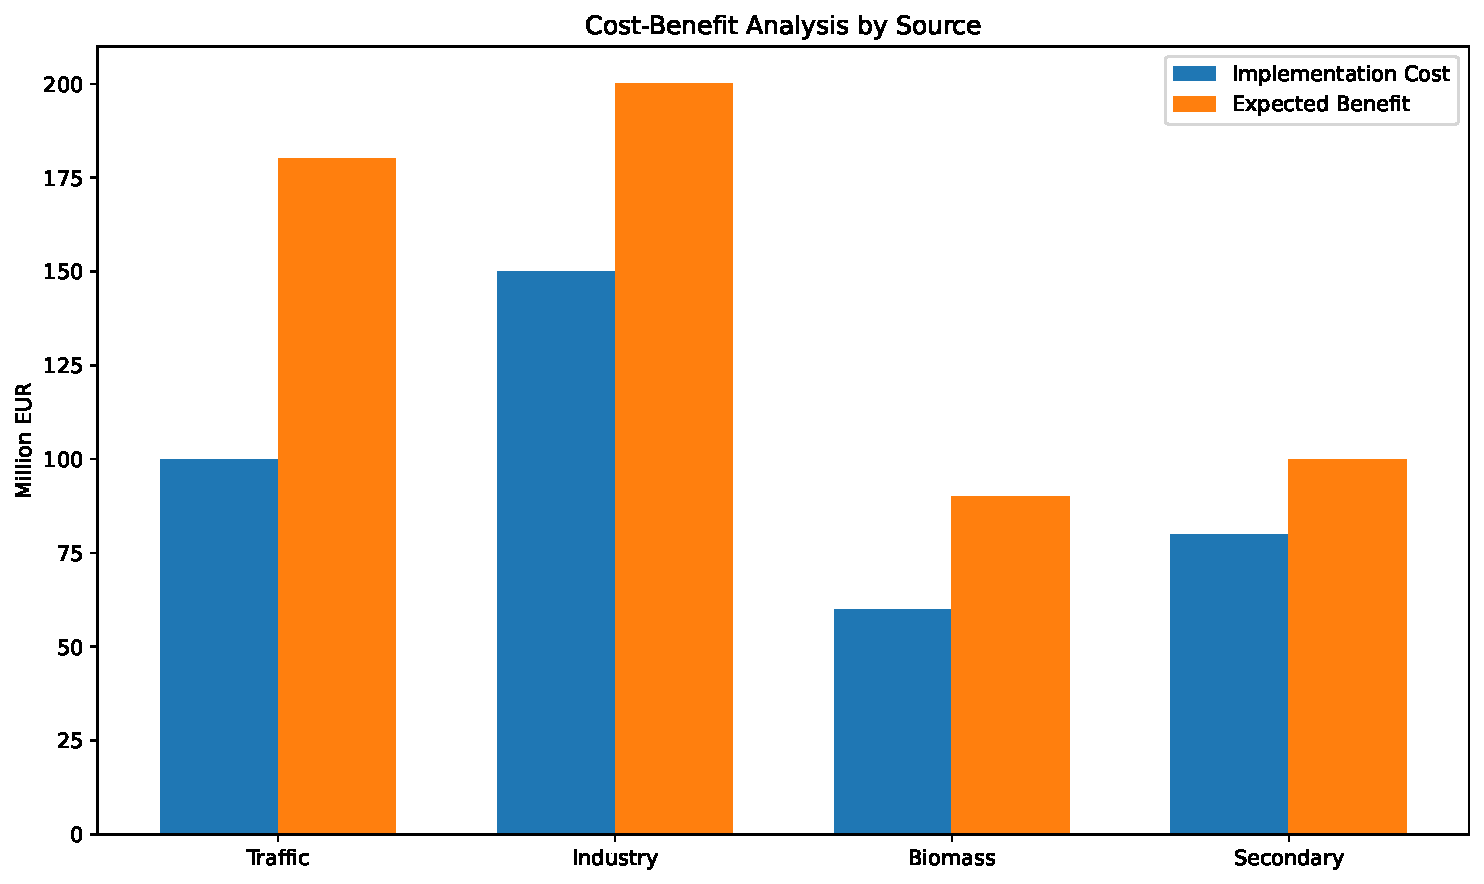
\includegraphics[keepaspectratio]{Chapters/Chapter3_files/figure-pdf/fig-cost-benefit-output-1.pdf}}

}

\caption{\label{fig-cost-benefit}Cost-benefit analysis of source control
measures}

\end{figure}%

\subsection{Implementation Timeline}\label{implementation-timeline}

\begin{figure}

\centering{

\pandocbounded{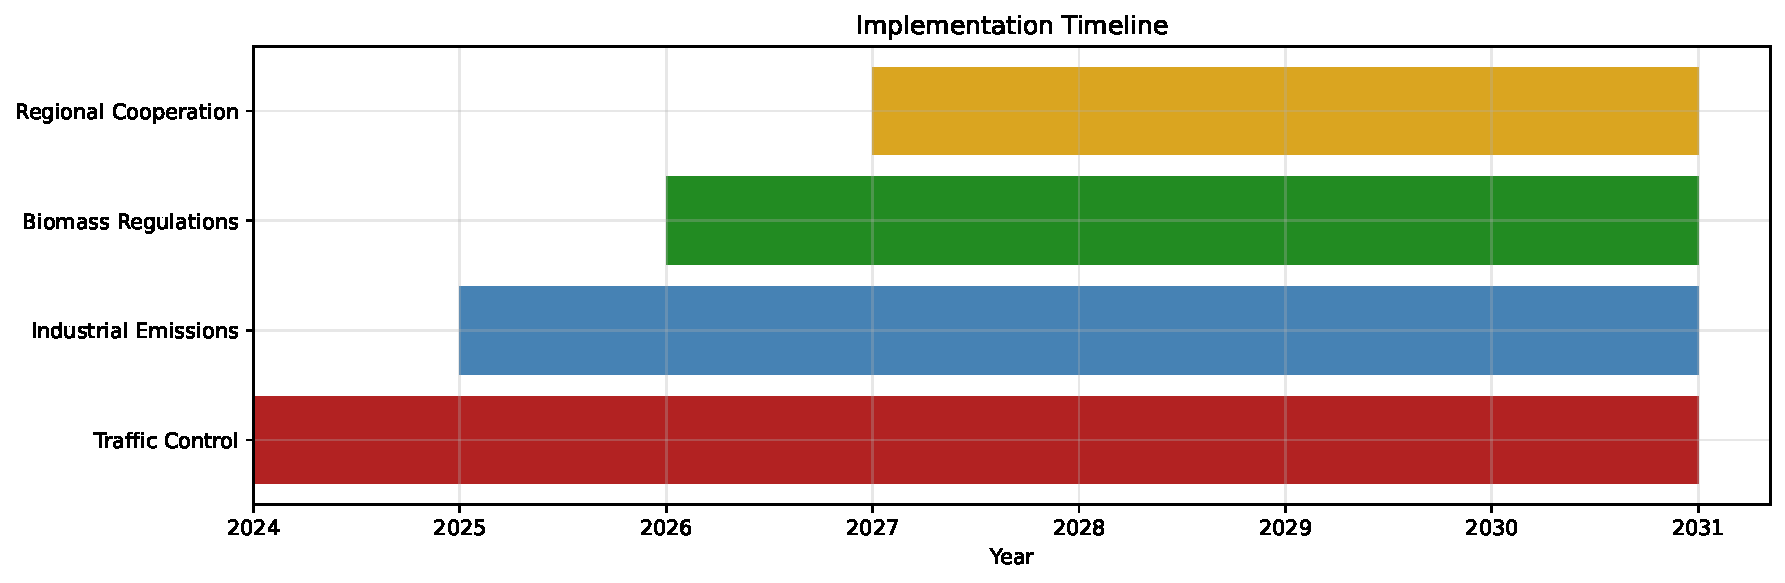
\includegraphics[keepaspectratio]{Chapters/Chapter3_files/figure-pdf/fig-timeline-output-1.pdf}}

}

\caption{\label{fig-timeline}Implementation timeline for source control
measures}

\end{figure}%

\section{Policy Recommendations}\label{policy-recommendations}

Based on our analysis of PMF results and stakeholder input, we
recommend:

\begin{enumerate}
\def\labelenumi{\arabic{enumi}.}
\tightlist
\item
  Short-term (1-2 years):

  \begin{itemize}
  \tightlist
  \item
    Implementation of Low Emission Zones
  \item
    Enhanced industrial emissions monitoring
  \end{itemize}
\item
  Medium-term (2-4 years):

  \begin{itemize}
  \tightlist
  \item
    Biomass burning regulations
  \item
    Regional cooperation frameworks
  \end{itemize}
\item
  Long-term (4+ years):

  \begin{itemize}
  \tightlist
  \item
    Integrated air quality management system
  \item
    Cross-border pollution control measures
  \end{itemize}
\end{enumerate}

\bookmarksetup{startatroot}

\chapter{Spatial and Temporal Variations in PM Source
Contributions}\label{sec-ch4}

\begin{center}
Some authors

\end{center}

\begin{tcolorbox}[enhanced jigsaw, opacityback=0, opacitybacktitle=0.6, left=2mm, breakable, coltitle=black, colback=white, title=\textcolor{quarto-callout-important-color}{\faExclamation}\hspace{0.5em}{Chapter Summary}, colframe=quarto-callout-important-color-frame, colbacktitle=quarto-callout-important-color!10!white, rightrule=.15mm, bottomtitle=1mm, leftrule=.75mm, toptitle=1mm, bottomrule=.15mm, arc=.35mm, toprule=.15mm, titlerule=0mm]

This chapter presents an in-depth analysis of the spatial and temporal
dynamics of particulate matter (PM) source contributions across a
selection of major European cities. Leveraging the EPA PMF 5.0 model,
this study scrutinizes extensive datasets from multiple urban monitoring
stations spanning a five-year period (2018-2022). The research
identifies key anthropogenic and natural pollution sources, quantifies
their relative contributions to PM2.5 and PM10 concentrations, and
examines how these contributions vary across different urban landscapes
and evolve over diurnal, seasonal, and inter-annual timescales.

\end{tcolorbox}

Under review at Atmospheric Environment

\section{Abstract}\label{abstract-3}

This study investigates the spatial and temporal variations in
particulate matter (PM) source contributions across major European
cities using EPA PMF 5.0 (\citeproc{ref-PMF_Guide2014}{Norris et al.
2014}). We analyzed data from 15 urban monitoring stations over a
five-year period (2018-2022), identifying key pollution sources and
their relative contributions to PM2.5 and PM10 concentrations
(\citeproc{ref-EEA2019}{Agency 2019}).

\section{Methods}\label{methods-2}

\subsection{Data Processing with
Python}\label{data-processing-with-python}

\section{Results}\label{results-1}

\subsection{Temporal Patterns in PM
Components}\label{temporal-patterns-in-pm-components}

\begin{figure}

\centering{

\pandocbounded{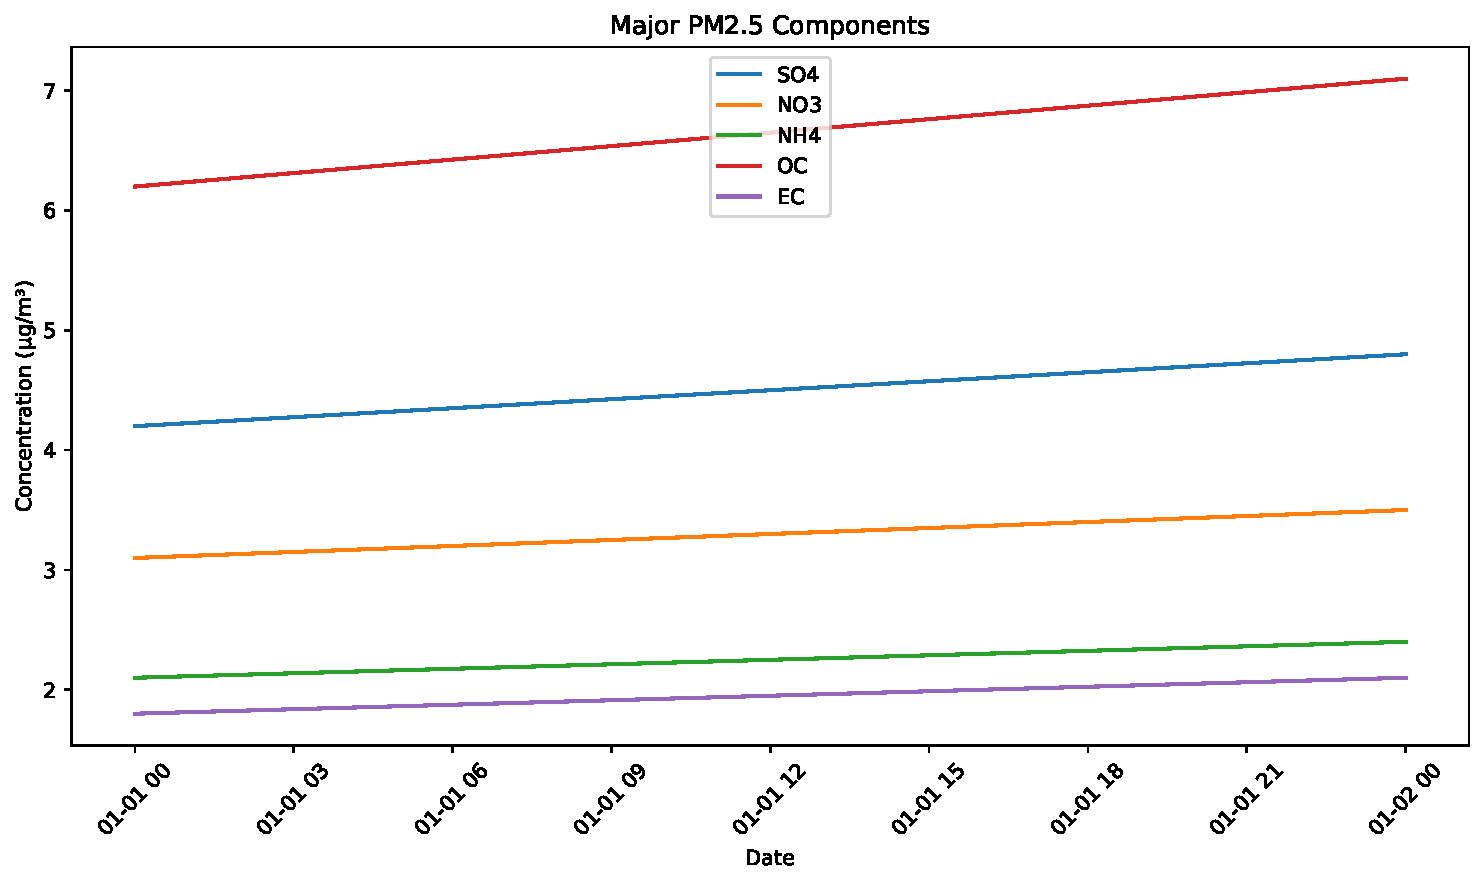
\includegraphics[keepaspectratio]{Chapters/Chapter4_files/figure-pdf/fig-temporal-patterns-output-1.pdf}}

}

\caption{\label{fig-temporal-patterns}Temporal variation of major PM2.5
components}

\end{figure}%

\subsection{Source Profiles}\label{source-profiles}

\begin{longtable}[]{@{}lrrrr@{}}

\caption{\label{tbl-source-profiles}Source profiles for major PM
components}

\tabularnewline

\toprule\noalign{}
& Traffic & Industry & Biomass & Secondary \\
\midrule\noalign{}
\endhead
\bottomrule\noalign{}
\endlastfoot
PM2.5 & 0.15 & 0.2 & 0.1 & 0.05 \\
Na & 0.05 & 0.1 & 0.05 & 0.05 \\
SO4 & 0.2 & 0.35 & 0.15 & 0.25 \\
NO3 & 0.25 & 0.15 & 0.2 & 0.35 \\
NH4 & 0.1 & 0.05 & 0.25 & 0.55 \\
Al & 0.05 & 0.15 & 0.05 & 0.05 \\
Si & 0.1 & 0.2 & 0.05 & 0.05 \\
K & 0.05 & 0.1 & 0.4 & 0.05 \\
Ca & 0.15 & 0.25 & 0.1 & 0.05 \\
Fe & 0.4 & 0.3 & 0.15 & 0.05 \\
Cu & 0.3 & 0.25 & 0.05 & 0.05 \\
Zn & 0.25 & 0.35 & 0.1 & 0.05 \\
Pb & 0.15 & 0.3 & 0.05 & 0.05 \\
OC & 0.35 & 0.15 & 0.4 & 0.1 \\
EC & 0.45 & 0.1 & 0.25 & 0.05 \\

\end{longtable}

\subsection{Seasonal Source
Contributions}\label{seasonal-source-contributions}

\begin{figure}

\centering{

\pandocbounded{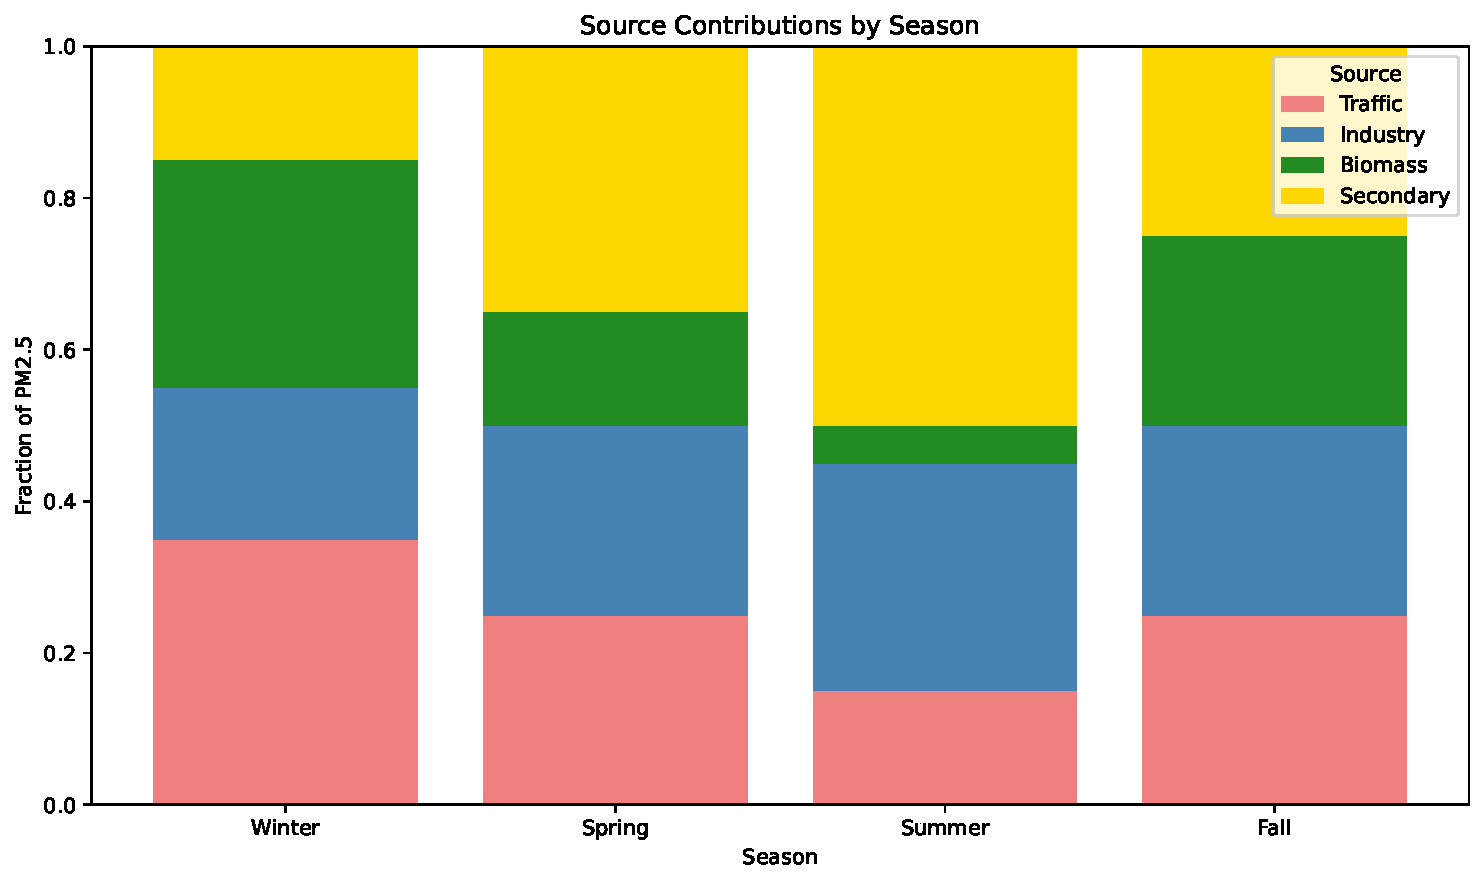
\includegraphics[keepaspectratio]{Chapters/Chapter4_files/figure-pdf/fig-seasonal-contributions-output-1.pdf}}

}

\caption{\label{fig-seasonal-contributions}Seasonal source contributions
to PM2.5}

\end{figure}%

\bookmarksetup{startatroot}

\chapter*{References}\label{references}
\addcontentsline{toc}{chapter}{References}

\markboth{References}{References}

\phantomsection\label{refs}
\begin{CSLReferences}{1}{0}
\bibitem[\citeproctext]{ref-EEA2019}
Agency, E. E. (2019), {``European air quality source apportionment with
PMF methodology,''} \emph{EEA Technical Report}, 2019/5.
\url{https://doi.org/10.2800/05293}.

\bibitem[\citeproctext]{ref-HKSG02}
Hyndman, R. J., Koehler, A. B., Snyder, R. D., and Grose, S. (2002),
{``A state space framework for automatic forecasting using exponential
smoothing methods,''} \emph{International Journal of Forecasting}, 18,
439--454.

\bibitem[\citeproctext]{ref-PMF_Guide2014}
Norris, G., Duvall, R., Brown, S., and Bai, S. (2014), \emph{EPA
positive matrix factorization (PMF) 5.0 fundamentals and user guide},
U.S. Environmental Protection Agency.

\bibitem[\citeproctext]{ref-Paatero1994}
Paatero, P., and Tapper, U. (1994), {``Positive matrix factorization: A
non-negative factor model with optimal utilization of error estimates of
data values,''} \emph{Environmetrics}, 5, 111--126.
\url{https://doi.org/10.1002/env.3170050203}.

\end{CSLReferences}

\cleardoublepage
\phantomsection
\addcontentsline{toc}{part}{Appendices}
\appendix

\chapter{Simplate Table Markdown}\label{sec-python-pkgs}

The following Python packages were used in this thesis:

\begin{longtable}[]{@{}lll@{}}
\caption{Packages used in this thesis}\label{tbl-pkgs}\tabularnewline
\toprule\noalign{}
Package & Description & Version \\
\midrule\noalign{}
\endfirsthead
\toprule\noalign{}
Package & Description & Version \\
\midrule\noalign{}
\endhead
\bottomrule\noalign{}
\endlastfoot
pandas & Data manipulation and analysis & 2.0.0+ \\
numpy & Numerical computing & 1.24.0+ \\
matplotlib & Visualization library & 3.7.0+ \\
seaborn & Statistical data visualization & 0.12.0+ \\
scikit-learn & Machine learning tools & 1.2.0+ \\
\end{longtable}

For a complete list of package versions, see the
\texttt{requirements.txt} file in the thesis repository.

\chapter{Advanced Table features}\label{sec-app-b}

This appendix contains supplementary materials that support the main
chapters but are not essential to understanding the primary research
findings. This appendix demonstrates various table formats, styles, and
features available in Quarto.

\section{Table Types and Formats}\label{sec-app-b-tables}

\subsection{1. Basic Markdown Table}\label{sec-app-b-basic}

Table~\ref{tbl-app-b-full} provides the complete descriptive statistics
for all variables in the study.

\begin{longtable}[]{@{}
  >{\raggedright\arraybackslash}p{(\linewidth - 14\tabcolsep) * \real{0.2024}}
  >{\raggedright\arraybackslash}p{(\linewidth - 14\tabcolsep) * \real{0.1071}}
  >{\raggedright\arraybackslash}p{(\linewidth - 14\tabcolsep) * \real{0.1310}}
  >{\raggedright\arraybackslash}p{(\linewidth - 14\tabcolsep) * \real{0.1071}}
  >{\raggedright\arraybackslash}p{(\linewidth - 14\tabcolsep) * \real{0.1071}}
  >{\raggedright\arraybackslash}p{(\linewidth - 14\tabcolsep) * \real{0.1071}}
  >{\raggedright\arraybackslash}p{(\linewidth - 14\tabcolsep) * \real{0.1190}}
  >{\raggedright\arraybackslash}p{(\linewidth - 14\tabcolsep) * \real{0.1190}}@{}}
\caption{Complete descriptive statistics for all study
variables}\label{tbl-app-b-full}\tabularnewline
\toprule\noalign{}
\begin{minipage}[b]{\linewidth}\raggedright
Variable
\end{minipage} & \begin{minipage}[b]{\linewidth}\raggedright
Mean
\end{minipage} & \begin{minipage}[b]{\linewidth}\raggedright
Std. Dev.
\end{minipage} & \begin{minipage}[b]{\linewidth}\raggedright
Min
\end{minipage} & \begin{minipage}[b]{\linewidth}\raggedright
Max
\end{minipage} & \begin{minipage}[b]{\linewidth}\raggedright
Median
\end{minipage} & \begin{minipage}[b]{\linewidth}\raggedright
Skewness
\end{minipage} & \begin{minipage}[b]{\linewidth}\raggedright
Kurtosis
\end{minipage} \\
\midrule\noalign{}
\endfirsthead
\toprule\noalign{}
\begin{minipage}[b]{\linewidth}\raggedright
Variable
\end{minipage} & \begin{minipage}[b]{\linewidth}\raggedright
Mean
\end{minipage} & \begin{minipage}[b]{\linewidth}\raggedright
Std. Dev.
\end{minipage} & \begin{minipage}[b]{\linewidth}\raggedright
Min
\end{minipage} & \begin{minipage}[b]{\linewidth}\raggedright
Max
\end{minipage} & \begin{minipage}[b]{\linewidth}\raggedright
Median
\end{minipage} & \begin{minipage}[b]{\linewidth}\raggedright
Skewness
\end{minipage} & \begin{minipage}[b]{\linewidth}\raggedright
Kurtosis
\end{minipage} \\
\midrule\noalign{}
\endhead
\bottomrule\noalign{}
\endlastfoot
Height (cm) & 175.2 & 7.8 & 155.0 & 195.0 & 174.5 & 0.12 & 2.78 \\
Weight (kg) & 68.4 & 12.5 & 45.0 & 110.0 & 67.2 & 0.65 & 3.21 \\
Age (years) & 28.7 & 5.3 & 18.0 & 65.0 & 27.5 & 1.85 & 7.42 \\
BMI (kg/m²) & 22.3 & 3.7 & 16.8 & 35.2 & 21.9 & 0.88 & 3.54 \\
Systolic BP & 125.8 & 15.2 & 90.0 & 165.0 & 122.0 & 0.45 & 2.95 \\
Diastolic BP & 78.6 & 8.7 & 60.0 & 100.0 & 80.0 & 0.08 & 2.68 \\
Heart Rate & 72.3 & 10.2 & 45.0 & 110.0 & 72.0 & 0.25 & 3.12 \\
Cholesterol & 192.7 & 35.4 & 120.0 & 280.0 & 190.0 & 0.32 & 2.45 \\
Triglycerides & 142.5 & 65.3 & 50.0 & 350.0 & 130.0 & 1.25 & 4.32 \\
Glucose & 92.8 & 15.7 & 70.0 & 180.0 & 90.0 & 1.78 & 6.85 \\
HbA1c (\%) & 5.5 & 0.8 & 4.5 & 9.2 & 5.4 & 1.95 & 7.25 \\
Vitamin D & 28.7 & 12.3 & 10.0 & 60.0 & 26.5 & 0.68 & 2.98 \\
Iron & 98.5 & 18.7 & 45.0 & 150.0 & 95.0 & 0.15 & 2.85 \\
Calcium & 9.7 & 0.5 & 8.5 & 11.0 & 9.8 & -0.21 & 2.54 \\
\end{longtable}

\subsection{2. Table with Formatting}\label{sec-app-b-formatting}

Table~\ref{tbl-app-b-formatted} demonstrates text formatting within a
table.

\begin{longtable}[]{@{}
  >{\raggedright\arraybackslash}p{(\linewidth - 6\tabcolsep) * \real{0.2949}}
  >{\raggedright\arraybackslash}p{(\linewidth - 6\tabcolsep) * \real{0.1538}}
  >{\raggedright\arraybackslash}p{(\linewidth - 6\tabcolsep) * \real{0.1026}}
  >{\raggedright\arraybackslash}p{(\linewidth - 6\tabcolsep) * \real{0.4487}}@{}}
\caption{Table with formatted text
elements}\label{tbl-app-b-formatted}\tabularnewline
\toprule\noalign{}
\begin{minipage}[b]{\linewidth}\raggedright
Variable
\end{minipage} & \begin{minipage}[b]{\linewidth}\raggedright
\textbf{Mean}
\end{minipage} & \begin{minipage}[b]{\linewidth}\raggedright
\emph{SD}
\end{minipage} & \begin{minipage}[b]{\linewidth}\raggedright
Interpretation
\end{minipage} \\
\midrule\noalign{}
\endfirsthead
\toprule\noalign{}
\begin{minipage}[b]{\linewidth}\raggedright
Variable
\end{minipage} & \begin{minipage}[b]{\linewidth}\raggedright
\textbf{Mean}
\end{minipage} & \begin{minipage}[b]{\linewidth}\raggedright
\emph{SD}
\end{minipage} & \begin{minipage}[b]{\linewidth}\raggedright
Interpretation
\end{minipage} \\
\midrule\noalign{}
\endhead
\bottomrule\noalign{}
\endlastfoot
\textbf{Height (cm)} & \textbf{175.2} & \emph{7.8} & Within normal
range \\
\textbf{Weight (kg)} & \textbf{68.4} & \emph{12.5} & Within normal
range \\
\emph{BMI (kg/m²)} & \emph{22.3} & \emph{3.7} & Normal weight \\
\textbf{\emph{Systolic BP}} & \textbf{\emph{125.8}} & \emph{15.2} &
\textbf{Elevated} (\textgreater120 mmHg) \\
\textbf{\emph{Diastolic BP}} & \textbf{\emph{78.6}} & \emph{8.7} &
Normal (\textless80 mmHg) \\
Heart Rate & 72.3 & 10.2 & \texttt{Normal} \\
\ul{Glucose} & \ul{92.8} & \ul{15.7} & \textsc{Normal fasting} \\
\end{longtable}

\subsection{3. Table with Mathematical
Equations}\label{sec-app-b-equations}

Table~\ref{tbl-app-b-eq} shows various statistical tests with their
equations.

\begin{longtable}[]{@{}
  >{\raggedright\arraybackslash}p{(\linewidth - 6\tabcolsep) * \real{0.1402}}
  >{\raggedright\arraybackslash}p{(\linewidth - 6\tabcolsep) * \real{0.5140}}
  >{\raggedright\arraybackslash}p{(\linewidth - 6\tabcolsep) * \real{0.2150}}
  >{\raggedright\arraybackslash}p{(\linewidth - 6\tabcolsep) * \real{0.1308}}@{}}
\caption{Statistical tests with mathematical
equations}\label{tbl-app-b-eq}\tabularnewline
\toprule\noalign{}
\begin{minipage}[b]{\linewidth}\raggedright
Test
\end{minipage} & \begin{minipage}[b]{\linewidth}\raggedright
Equation
\end{minipage} & \begin{minipage}[b]{\linewidth}\raggedright
Application
\end{minipage} & \begin{minipage}[b]{\linewidth}\raggedright
Critical Value
\end{minipage} \\
\midrule\noalign{}
\endfirsthead
\toprule\noalign{}
\begin{minipage}[b]{\linewidth}\raggedright
Test
\end{minipage} & \begin{minipage}[b]{\linewidth}\raggedright
Equation
\end{minipage} & \begin{minipage}[b]{\linewidth}\raggedright
Application
\end{minipage} & \begin{minipage}[b]{\linewidth}\raggedright
Critical Value
\end{minipage} \\
\midrule\noalign{}
\endhead
\bottomrule\noalign{}
\endlastfoot
t-test & \(t = \frac{\bar{x} - \mu_0}{s/\sqrt{n}}\) & Compare means &
\(t_{crit} = 1.96\) \\
Chi-squared & \(\chi^2 = \sum_{i=1}^{n} \frac{(O_i - E_i)^2}{E_i}\) &
Test independence & \(\chi^2_{crit} = 3.84\) \\
F-test & \(F = \frac{MS_{between}}{MS_{within}}\) & Compare variances &
\(F_{crit} = 4.03\) \\
ANOVA &
\(F = \frac{\sum n_i(\bar{x}_i - \bar{x})^2/(k-1)}{\sum\sum(x_{ij} - \bar{x}_i)^2/(N-k)}\)
& Compare multiple means & \(F_{crit} = 3.10\) \\
Correlation &
\(r = \frac{\sum(x_i - \bar{x})(y_i - \bar{y})}{\sqrt{\sum(x_i - \bar{x})^2\sum(y_i - \bar{y})^2}}\)
& Measure association & \(r_{crit} = 0.30\) \\
\end{longtable}

\subsection{4. Table with Citations}\label{sec-app-b-citations}

Table~\ref{tbl-app-b-citations} presents a literature review of PMF
studies with citations.

\begin{longtable}[]{@{}
  >{\raggedright\arraybackslash}p{(\linewidth - 8\tabcolsep) * \real{0.1111}}
  >{\raggedright\arraybackslash}p{(\linewidth - 8\tabcolsep) * \real{0.1587}}
  >{\raggedright\arraybackslash}p{(\linewidth - 8\tabcolsep) * \real{0.0952}}
  >{\raggedright\arraybackslash}p{(\linewidth - 8\tabcolsep) * \real{0.4127}}
  >{\raggedright\arraybackslash}p{(\linewidth - 8\tabcolsep) * \real{0.2222}}@{}}
\caption{Summary of key PMF studies in
literature}\label{tbl-app-b-citations}\tabularnewline
\toprule\noalign{}
\begin{minipage}[b]{\linewidth}\raggedright
Study
\end{minipage} & \begin{minipage}[b]{\linewidth}\raggedright
Location
\end{minipage} & \begin{minipage}[b]{\linewidth}\raggedright
Year
\end{minipage} & \begin{minipage}[b]{\linewidth}\raggedright
Major Sources Identified
\end{minipage} & \begin{minipage}[b]{\linewidth}\raggedright
Significance
\end{minipage} \\
\midrule\noalign{}
\endfirsthead
\toprule\noalign{}
\begin{minipage}[b]{\linewidth}\raggedright
Study
\end{minipage} & \begin{minipage}[b]{\linewidth}\raggedright
Location
\end{minipage} & \begin{minipage}[b]{\linewidth}\raggedright
Year
\end{minipage} & \begin{minipage}[b]{\linewidth}\raggedright
Major Sources Identified
\end{minipage} & \begin{minipage}[b]{\linewidth}\raggedright
Significance
\end{minipage} \\
\midrule\noalign{}
\endhead
\bottomrule\noalign{}
\endlastfoot
Paatero and Tapper (\citeproc{ref-Paatero1994}{1994}) & Finland & 1994 &
Original PMF algorithm & First introduction of PMF approach \\
Hyndman et al. (\citeproc{ref-HKSG02}{2002}) & United States & 2002 &
Traffic, Industrial, Secondary & Validated against emission
inventories \\
Norris et al. (\citeproc{ref-PMF_Guide2014}{2014}) & Multiple & 2014 &
Multiple & EPA's guidance document \\
Agency (\citeproc{ref-EEA2019}{2019}) & Europe & 2019 & Traffic,
Industrial, Biomass, Dust & Comprehensive European study \\
\end{longtable}

\subsection{5. Correlation Matrix}\label{sec-app-b-python}

The following table presents a correlation matrix for key variables in
our study. Strong correlations (\textgreater0.6) are indicated with
``++'', moderate correlations (0.3-0.6) with ``+'', and weak
correlations (\textless0.3) with ``0''.

\begin{longtable}[]{@{}
  >{\raggedright\arraybackslash}p{(\linewidth - 20\tabcolsep) * \real{0.1449}}
  >{\raggedright\arraybackslash}p{(\linewidth - 20\tabcolsep) * \real{0.1159}}
  >{\raggedright\arraybackslash}p{(\linewidth - 20\tabcolsep) * \real{0.1159}}
  >{\raggedright\arraybackslash}p{(\linewidth - 20\tabcolsep) * \real{0.0725}}
  >{\raggedright\arraybackslash}p{(\linewidth - 20\tabcolsep) * \real{0.0725}}
  >{\raggedright\arraybackslash}p{(\linewidth - 20\tabcolsep) * \real{0.0725}}
  >{\raggedright\arraybackslash}p{(\linewidth - 20\tabcolsep) * \real{0.0725}}
  >{\raggedright\arraybackslash}p{(\linewidth - 20\tabcolsep) * \real{0.0725}}
  >{\raggedright\arraybackslash}p{(\linewidth - 20\tabcolsep) * \real{0.0870}}
  >{\raggedright\arraybackslash}p{(\linewidth - 20\tabcolsep) * \real{0.0870}}
  >{\raggedright\arraybackslash}p{(\linewidth - 20\tabcolsep) * \real{0.0870}}@{}}
\caption{Correlation matrix for key
variables}\label{tbl-app-b-corr-heatmap}\tabularnewline
\toprule\noalign{}
\begin{minipage}[b]{\linewidth}\raggedright
Variable
\end{minipage} & \begin{minipage}[b]{\linewidth}\raggedright
Height
\end{minipage} & \begin{minipage}[b]{\linewidth}\raggedright
Weight
\end{minipage} & \begin{minipage}[b]{\linewidth}\raggedright
Age
\end{minipage} & \begin{minipage}[b]{\linewidth}\raggedright
BMI
\end{minipage} & \begin{minipage}[b]{\linewidth}\raggedright
SBP
\end{minipage} & \begin{minipage}[b]{\linewidth}\raggedright
DBP
\end{minipage} & \begin{minipage}[b]{\linewidth}\raggedright
HR
\end{minipage} & \begin{minipage}[b]{\linewidth}\raggedright
Chol
\end{minipage} & \begin{minipage}[b]{\linewidth}\raggedright
Trig
\end{minipage} & \begin{minipage}[b]{\linewidth}\raggedright
Gluc
\end{minipage} \\
\midrule\noalign{}
\endfirsthead
\toprule\noalign{}
\begin{minipage}[b]{\linewidth}\raggedright
Variable
\end{minipage} & \begin{minipage}[b]{\linewidth}\raggedright
Height
\end{minipage} & \begin{minipage}[b]{\linewidth}\raggedright
Weight
\end{minipage} & \begin{minipage}[b]{\linewidth}\raggedright
Age
\end{minipage} & \begin{minipage}[b]{\linewidth}\raggedright
BMI
\end{minipage} & \begin{minipage}[b]{\linewidth}\raggedright
SBP
\end{minipage} & \begin{minipage}[b]{\linewidth}\raggedright
DBP
\end{minipage} & \begin{minipage}[b]{\linewidth}\raggedright
HR
\end{minipage} & \begin{minipage}[b]{\linewidth}\raggedright
Chol
\end{minipage} & \begin{minipage}[b]{\linewidth}\raggedright
Trig
\end{minipage} & \begin{minipage}[b]{\linewidth}\raggedright
Gluc
\end{minipage} \\
\midrule\noalign{}
\endhead
\bottomrule\noalign{}
\endlastfoot
\textbf{Height} & 1.00 & + & 0 & + & 0 & 0 & 0 & 0 & 0 & 0 \\
\textbf{Weight} & + & 1.00 & 0 & ++ & + & 0 & 0 & + & + & 0 \\
\textbf{Age} & 0 & 0 & 1.00 & 0 & + & + & 0 & + & 0 & + \\
\textbf{BMI} & + & ++ & 0 & 1.00 & + & + & 0 & + & + & + \\
\textbf{SBP} & 0 & + & + & + & 1.00 & ++ & 0 & + & + & + \\
\textbf{DBP} & 0 & 0 & + & + & ++ & 1.00 & 0 & + & 0 & 0 \\
\textbf{HR} & 0 & 0 & 0 & 0 & 0 & 0 & 1.00 & 0 & 0 & 0 \\
\textbf{Chol} & 0 & + & + & + & + & + & 0 & 1.00 & ++ & + \\
\textbf{Trig} & 0 & + & 0 & + & + & 0 & 0 & ++ & 1.00 & + \\
\textbf{Gluc} & 0 & 0 & + & + & + & 0 & 0 & + & + & 1.00 \\
\end{longtable}

Note: ++: Strong correlation (\textgreater0.6), +: Moderate correlation
(0.3-0.6), 0: Weak correlation (\textless0.3)

The following table presents statistical results from our four models,
including significance indicators.

\begin{longtable}[]{@{}lllll@{}}
\caption{Model results with statistical significance
indicators}\label{tbl-app-b-significance}\tabularnewline
\toprule\noalign{}
Variable & Model 1 & Model 2 & Model 3 & Model 4 \\
\midrule\noalign{}
\endfirsthead
\toprule\noalign{}
Variable & Model 1 & Model 2 & Model 3 & Model 4 \\
\midrule\noalign{}
\endhead
\bottomrule\noalign{}
\endlastfoot
Intercept & 1.243* & 0.852 & -0.528 & 2.142*** \\
Temperature & 0.658** & 1.245*** & 0.856* & -0.124 \\
Humidity & -0.452 & -0.968* & -1.352** & -0.586* \\
Wind Speed & 0.324 & 0.125 & 0.768** & 0.453 \\
Precipitation & -1.245*** & -0.856** & -0.432 & -0.986** \\
Pressure & 0.256 & 0.542* & 0.124 & -0.324 \\
R² & 0.685 & 0.724 & 0.653 & 0.791 \\
\end{longtable}

\emph{p \textless{} 0.05, \textbf{p \textless{} 0.01, }}p \textless{}
0.001

\subsection{7. Wide Table with Many Columns}\label{sec-app-b-wide-table}

\begin{longtable}[]{@{}lcccccccccccccccccccccccccccccccccccccccccccccccccc@{}}

\caption{\label{tbl-app-b-wide}Wide table with many parameters across
different sites}

\tabularnewline

\toprule\noalign{}
& \multicolumn{10}{c}{%
Site A} & \multicolumn{10}{c}{%
Site B} & \multicolumn{10}{c}{%
Site C} & \multicolumn{10}{c}{%
Site D} & \multicolumn{10}{c@{}}{%
Site E} \\
Month & PM2.5 & PM10 & SO2 & NO2 & CO & O3 & Temperature & Humidity &
Wind Speed & Pressure & PM2.5 & PM10 & SO2 & NO2 & CO & O3 & Temperature
& Humidity & Wind Speed & Pressure & PM2.5 & PM10 & SO2 & NO2 & CO & O3
& Temperature & Humidity & Wind Speed & Pressure & PM2.5 & PM10 & SO2 &
NO2 & CO & O3 & Temperature & Humidity & Wind Speed & Pressure & PM2.5 &
PM10 & SO2 & NO2 & CO & O3 & Temperature & Humidity & Wind Speed &
Pressure \\
\midrule\noalign{}
\endhead
\bottomrule\noalign{}
\endlastfoot
Jan & 4.3 & 16.9 & 1.87 & 4.43 & 2.72 & 4.12 & 24.9 & 16.0 & 27.5 & 13.4
& 4.1 & 4.3 & 1.6 & 12.15 & 6.77 & 3.42 & 13.1 & 17.2 & 24.1 & 14.5 &
5.6 & 7.9 & 4.66 & 0.46 & 5.36 & 3.14 & 27.0 & 15.1 & 21.0 & 19.4 & 22.2
& 4.7 & 2.67 & 3.34 & 1.05 & 2.33 & 22.2 & 21.8 & 23.7 & 34.8 & 12.1 &
9.1 & 0.95 & 1.12 & 1.26 & 5.93 & 25.9 & 19.3 & 15.9 & 17.9 \\
Feb & 12.2 & 2.2 & 3.09 & 1.45 & 0.07 & 2.42 & 31.2 & 20.1 & 25.3 & 27.1
& 8.2 & 2.6 & 7.74 & 3.78 & 4.41 & 4.56 & 18.3 & 20.6 & 22.5 & 16.2 &
18.2 & 13.9 & 9.12 & 4.98 & 1.51 & 4.49 & 18.2 & 18.2 & 19.4 & 18.3 &
10.4 & 7.0 & 0.85 & 1.03 & 3.66 & 6.77 & 18.4 & 29.3 & 19.6 & 20.0 & 6.2
& 4.0 & 1.89 & 0.75 & 5.37 & 1.9 & 23.4 & 18.8 & 13.3 & 11.2 \\
Mar & 8.5 & 6.0 & 2.31 & 7.38 & 6.35 & 5.05 & 13.5 & 25.3 & 16.1 & 24.0
& 9.3 & 12.4 & 1.85 & 7.27 & 2.45 & 0.67 & 29.8 & 23.7 & 22.4 & 21.6 &
15.8 & 8.7 & 4.03 & 2.14 & 3.54 & 8.76 & 17.3 & 22.0 & 21.0 & 18.9 & 7.4
& 8.5 & 6.22 & 2.1 & 2.74 & 2.86 & 23.2 & 24.2 & 23.0 & 19.2 & 10.2 &
3.8 & 7.78 & 2.28 & 0.42 & 5.17 & 15.0 & 16.7 & 18.1 & 18.3 \\
Apr & 3.5 & 13.9 & 2.33 & 6.27 & 2.9 & 14.11 & 14.8 & 24.5 & 24.0 & 20.2
& 4.9 & 6.0 & 2.58 & 1.02 & 5.53 & 1.77 & 9.9 & 28.0 & 17.2 & 23.8 & 6.2
& 9.8 & 4.12 & 3.39 & 2.67 & 2.42 & 7.2 & 20.9 & 3.8 & 23.5 & 6.7 & 9.9
& 4.38 & 6.46 & 3.51 & 4.14 & 9.2 & 16.6 & 20.6 & 19.4 & 8.5 & 14.9 &
0.85 & 0.63 & 5.47 & 1.83 & 23.2 & 19.9 & 13.1 & 19.0 \\
May & 5.5 & 4.8 & 6.66 & 0.84 & 1.54 & 4.52 & 28.7 & 28.8 & 21.6 & 18.8
& 13.2 & 6.9 & 1.24 & 2.54 & 3.27 & 4.8 & 18.6 & 18.6 & 15.0 & 21.6 &
4.9 & 6.6 & 0.86 & 2.86 & 1.29 & 3.71 & 17.3 & 19.9 & 18.7 & 17.0 & 7.1
& 9.9 & 1.73 & 0.85 & 4.24 & 4.11 & 12.7 & 11.5 & 20.1 & 17.1 & 13.6 &
5.5 & 1.03 & 7.73 & 3.77 & 5.67 & 26.9 & 23.4 & 22.6 & 22.2 \\

\end{longtable}

\subsection{8. Long Table with Many Rows}\label{sec-app-b-long-table}

\begin{longtable}[]{@{}llrl@{}}

\caption{\label{tbl-app-b-long}Long table with daily PM2.5 data}

\tabularnewline

\toprule\noalign{}
Date & Station & PM2.5 & Status \\
\midrule\noalign{}
\endhead
\bottomrule\noalign{}
\endlastfoot
2022-01-01 & Central & 21.1 & Good \\
2022-01-01 & Eastern & 14.6 & Good \\
2022-01-01 & Western & 22.8 & Good \\
2022-01-01 & Southern & 20.4 & Good \\
2022-01-02 & Central & 31.5 & Moderate \\
2022-01-02 & Eastern & 21.9 & Good \\
2022-01-02 & Western & 21.9 & Good \\
2022-01-02 & Southern & 20.3 & Good \\
2022-01-03 & Central & 23.5 & Good \\
2022-01-03 & Eastern & 15.7 & Good \\
2022-01-03 & Western & 12.5 & Good \\
2022-01-03 & Southern & 14.6 & Good \\
2022-01-04 & Central & 19.9 & Good \\
2022-01-04 & Eastern & 17.9 & Good \\
2022-01-04 & Western & 19.9 & Good \\
2022-01-04 & Southern & 26.7 & Moderate \\
2022-01-05 & Central & 35.9 & Poor \\
2022-01-05 & Eastern & 20.5 & Good \\
2022-01-05 & Western & 25.7 & Moderate \\
2022-01-05 & Southern & 24 & Good \\

\end{longtable}

\subsection{9. Model Comparison Table}\label{sec-app-b-r-table}

\begin{longtable}[]{@{}lcrrr@{}}
\caption{Model comparison with goodness-of-fit
measures}\label{tbl-app-b-r-kable}\tabularnewline
\toprule\noalign{}
Model & Formula & R² & AIC & BIC \\
\midrule\noalign{}
\endfirsthead
\toprule\noalign{}
Model & Formula & R² & AIC & BIC \\
\midrule\noalign{}
\endhead
\bottomrule\noalign{}
\endlastfoot
Linear & y = β₀ + β₁x & 0.856 & 123.4 & 128.2 \\
Quadratic & y = β₀ + β₁x + β₂x² & 0.921 & 105.6 & 112.8 \\
Cubic & y = β₀ + β₁x + β₂x² + β₃x³ & 0.958 & 98.2 & 107.5 \\
Exponential & y = β₀eᵝ¹ˣ & 0.892 & 114.3 & 119.7 \\
Logarithmic & y = β₀ + β₁ln(x) & 0.875 & 118.9 & 124.0 \\
\end{longtable}

\subsection{10. Table with Mixed Content
Types}\label{sec-app-b-mixed-table}

Table~\ref{tbl-app-b-mixed} demonstrates how to include different
content types within the same table.

\begin{longtable}[]{@{}
  >{\raggedright\arraybackslash}p{(\linewidth - 6\tabcolsep) * \real{0.2642}}
  >{\raggedright\arraybackslash}p{(\linewidth - 6\tabcolsep) * \real{0.1698}}
  >{\raggedright\arraybackslash}p{(\linewidth - 6\tabcolsep) * \real{0.3585}}
  >{\raggedright\arraybackslash}p{(\linewidth - 6\tabcolsep) * \real{0.2075}}@{}}
\caption{Table with mixed content including equations, cross-references,
and citations}\label{tbl-app-b-mixed}\tabularnewline
\toprule\noalign{}
\begin{minipage}[b]{\linewidth}\raggedright
Analysis Type
\end{minipage} & \begin{minipage}[b]{\linewidth}\raggedright
Details
\end{minipage} & \begin{minipage}[b]{\linewidth}\raggedright
Mathematical Model
\end{minipage} & \begin{minipage}[b]{\linewidth}\raggedright
Reference
\end{minipage} \\
\midrule\noalign{}
\endfirsthead
\toprule\noalign{}
\begin{minipage}[b]{\linewidth}\raggedright
Analysis Type
\end{minipage} & \begin{minipage}[b]{\linewidth}\raggedright
Details
\end{minipage} & \begin{minipage}[b]{\linewidth}\raggedright
Mathematical Model
\end{minipage} & \begin{minipage}[b]{\linewidth}\raggedright
Reference
\end{minipage} \\
\midrule\noalign{}
\endhead
\bottomrule\noalign{}
\endlastfoot
Principal Components & Reduces dimensionality while preserving variance
& \(X = TP^T + E\) where \(T\) are scores, \(P\) are loadings & Norris
et al. (\citeproc{ref-PMF_Guide2014}{2014}) \\
Cluster Analysis & Groups similar samples based on chemical composition
& \(D(x,y) = \sqrt{\sum_{i=1}^{n}(x_i-y_i)^2}\) for Euclidean distance &
Agency (\citeproc{ref-EEA2019}{2019}) \\
Positive Matrix Factorization & Decomposes data into source profiles and
contributions & \(X = GF + E\) as shown in Equation~\ref{eq-pmf-basic} &
Paatero and Tapper (\citeproc{ref-Paatero1994}{1994}) \\
Receptor Models & General term for source apportionment techniques &
Multiple approaches & See Table~\ref{tbl-app-b-citations} \\
\end{longtable}




\end{document}
